\documentclass[]{article}
\usepackage{lmodern}
\usepackage{amssymb,amsmath}
\usepackage{ifxetex,ifluatex}
\usepackage{fixltx2e} % provides \textsubscript
\ifnum 0\ifxetex 1\fi\ifluatex 1\fi=0 % if pdftex
  \usepackage[T1]{fontenc}
  \usepackage[utf8]{inputenc}
\else % if luatex or xelatex
  \ifxetex
    \usepackage{mathspec}
  \else
    \usepackage{fontspec}
  \fi
  \defaultfontfeatures{Ligatures=TeX,Scale=MatchLowercase}
\fi
% use upquote if available, for straight quotes in verbatim environments
\IfFileExists{upquote.sty}{\usepackage{upquote}}{}
% use microtype if available
\IfFileExists{microtype.sty}{%
\usepackage{microtype}
\UseMicrotypeSet[protrusion]{basicmath} % disable protrusion for tt fonts
}{}
\usepackage[margin=1in]{geometry}
\usepackage{hyperref}
\hypersetup{unicode=true,
            pdfborder={0 0 0},
            breaklinks=true}
\urlstyle{same}  % don't use monospace font for urls
\usepackage{graphicx,grffile}
\makeatletter
\def\maxwidth{\ifdim\Gin@nat@width>\linewidth\linewidth\else\Gin@nat@width\fi}
\def\maxheight{\ifdim\Gin@nat@height>\textheight\textheight\else\Gin@nat@height\fi}
\makeatother
% Scale images if necessary, so that they will not overflow the page
% margins by default, and it is still possible to overwrite the defaults
% using explicit options in \includegraphics[width, height, ...]{}
\setkeys{Gin}{width=\maxwidth,height=\maxheight,keepaspectratio}
\IfFileExists{parskip.sty}{%
\usepackage{parskip}
}{% else
\setlength{\parindent}{0pt}
\setlength{\parskip}{6pt plus 2pt minus 1pt}
}
\setlength{\emergencystretch}{3em}  % prevent overfull lines
\providecommand{\tightlist}{%
  \setlength{\itemsep}{0pt}\setlength{\parskip}{0pt}}
\setcounter{secnumdepth}{0}
% Redefines (sub)paragraphs to behave more like sections
\ifx\paragraph\undefined\else
\let\oldparagraph\paragraph
\renewcommand{\paragraph}[1]{\oldparagraph{#1}\mbox{}}
\fi
\ifx\subparagraph\undefined\else
\let\oldsubparagraph\subparagraph
\renewcommand{\subparagraph}[1]{\oldsubparagraph{#1}\mbox{}}
\fi

%%% Use protect on footnotes to avoid problems with footnotes in titles
\let\rmarkdownfootnote\footnote%
\def\footnote{\protect\rmarkdownfootnote}

%%% Change title format to be more compact
\usepackage{titling}

% Create subtitle command for use in maketitle
\newcommand{\subtitle}[1]{
  \posttitle{
    \begin{center}\large#1\end{center}
    }
}

\setlength{\droptitle}{-2em}

  \title{}
    \pretitle{\vspace{\droptitle}}
  \posttitle{}
    \author{}
    \preauthor{}\postauthor{}
    \date{}
    \predate{}\postdate{}
  

\begin{document}

\chapter[Renfrewshire Council Exploratory Project]{Renfrewshire Council \\ Exploratory Project}\label{ch:renfrew}

\thispagestyle{empty}

\section{Introduction}\label{renf-intro}

As described in Section \ref{subsec:source-sc}, the Social Care Survey
(SCS) is collected annually by the Scottish Government and provides
information on the types and amounts of social care delivered to
individuals in all 32 Scottish local authorities. This information is
collected in two ways depending on which service an individual may
receive. The most recent surveys collect data on all individuals who
receive a community alarm service, a telecare service,
self-directed-support payments, or assistance via a social or support
worker at any time during the financial year. Home care, housing
support, and meals (hereafter referred to collectively as ``home care'')
data is collected only for individuals receiving these services during a
census week - usually including the date 31\textsuperscript{st} March
(Scottish-Government 2017c). The cross-sectional nature of the data
collected for these second group of services means that the SCS does not
identify every individual who receives social care in any given
financial year. This has implications for the interpretation of research
projects using the SCS and the statistical inferences that can be
applied to the data when linked with other sources of information. This
chapter estimates the numbers of individuals receiving home care
``missed'' by the SCS, their demographic make-up, and the type of care
they received by analysing complete data from one local authority area.
It also identifes how many more individuals receiving home care would be
identified by the SCS if a census quarter, rather than cenus week, was
implemented.

All data relating to home care services from Renfrewshire council was
de-identified and transferred securely to a safe haven environment to
enable analyses. Information of differing types of home care services
were summarised and a weekly time series indicating the amount of
service provision in each week was created for the period April
2006-March 2016.

Over the study period, between ?\% and ?\% of all indiviudals receiving
home care in each financial year received home care during the census
week. This percentage would increase by approximately 10\% if a
quarterly census were implemented. There were no major differences in
age and sex between those ``missed'' and ``caught'' by the SCS. However,
those missed etc.etc.

Implications

\section{Background}\label{sec:renf-background}

Two reasons that individuals may receive home care services but not be
captured by the SCS include death before the census week and receipt of
short-term home care services. Whilst it is difficult to quantify
numbers of people who fall into the former category, this chapter
provides some insight into levels of the latter. Given intentions to
amalgamate the SCS with administrative resources collected by ISD and
move to a quarterly collection of data (ISD 2017), the exploratory
project also aimed to quantify the percentage of all individuals that
would be identified by collection of home care data in quarter 4 of each
financial year (this quarter is the proposed time period for collection
of the 2017/18 census).

As social care data in Scotland has rarely been used for research
purposes, this exploratory project also offered the opportunity to
assess the format, content, and suitability of the data from a research
perspective. Ideally, data would be analysed from a number of local
authorities for comparison. However, as described below, acquiring
sensitive data of this nature is a lengthy and complicated process,
relying heavily on the goodwill of the participating local authority.
Despite early intentions to approach multiple local authorities,
practical considerations limited the project to data collected from
Renfrewshire Council.

The decision to approach Renfrewshire Council as a potential source of
data was due to convenience given previous cooperation between the
council and UBDC on other projects. Another local authority was also
approached but preliminary discussions suggested that whilst the purpose
of proposed research was supported, the council was unlikely to be able
to provide sufficient resource to facilitate data sharing. Preliminary
meetings with data analysts from Renfrewshire council confirmed that
data could be provided to facilitate the proposed research and the
formal process of obtaining data using UBDC's controlled data service
was instigated in April 2016.

Despite there only being a single source of data, Renfrewshire Council
offers an excellent location in which to explore the receipt of social
care given it is fairly representative of Scotland as a whole. It is the
10\textsuperscript{th} largest local authority in Scotland with 3.2\% of
the total population of the country. It has a similar proportion of
individuals aged over 60 compared to the rest of the country (24.4\% v
24.2\%) (NRS 2015) and the mortality rate is only slightly higher than
recorded for the rest of Scotland (10.9\% v 10.3\%). Some of the most
and least deprived datazones in the whole of Scotland are present in
Renfrewshire and a spread of urban and rural neighbourhoods
(Scottish-Government 2017a) (see also figure \ref{fig:results1-la} which
indicates a very even spread of individuals over 65 in all ten SIMD
deciles).

In terms of social care, the 2017 SCS (Scottish-Government 2017b,
supp.charts) shows that the proportion of over 65s receiving home care
provided or administered by Renfrewshire Council dipped a little between
2011 and 2015 but has nearly returned to 2010 levels (52.4 per thousand
in 2010, 49.4 per thousand in 2017). Historically, this is lower than
levels seen across Scotland as a whole, although national levels are now
very similar to those seen in Renfrewshire (60.8 per thousand in 2010 to
48.9 per thousand in 2017). Absolute numbers of over 65s receiving home
care in Renfrewshire in the 2010 census week was 1526 versus 1614 in the
2017 census (Scottish-Government 2017b, supp.charts).

b \textbf{Bit (again) about the data collected in census week then
mention split in home care for table}

Home care refers to services received in the home such as personal care
or reablement (described in section \ref{subsec:access-sc-defs} and
summarised in table \ref{tab:renf-homecaredefs}).

\rowcolors{2}{gray!25}{white}

\begin{table}[]
\centering
\resizebox{\textwidth}{!}{%
\begin{tabular}{@{}ll@{}}
\toprule
\textbf{Type of home care} & \textbf{Definition} \\ \midrule
Care at Home (Mainstream & \begin{tabular}[c]{@{}l@{}}The aim of care at home is to help vulnerable people of all ages live independently and securely in their\\  own homes by providing personal and housing support services. Care at home services are provided very\\  much on each individual's own circumstances and needs.\end{tabular} \\ \midrule
Reablement & \begin{tabular}[c]{@{}l@{}}Provides support and encouragement to help keep up or increase the skills and confidence needed \\ to be able to return home after a stay in hospital or after an illness.Most people referred for care at \\ home will receive a reablement service in the first instance to help support and improve independence.\\ Long term services can be provided following reablement if ongoing support is needed.\end{tabular} \\ \midrule
Rapid Response & \begin{tabular}[c]{@{}l@{}}Rapid intervention care at home aimed at preventing hospital admissions ot facilitating hospital discharges\\ while longer term care packages are put in place. \end{tabular} \\ \midrule
Community Mental Health & \begin{tabular}[c]{@{}l@{}}Care at home service designed to supprt service users of the Community Mental Health team to live\\ independently in the community\end{tabular} \\ \midrule
Extra Care Housing &  Care at home based on site for tenents of Local Authority extra care housing complexes\\ \midrule
Housing Support & Care at home services to support service users to maintain tenancies and live independently in the community\\ \midrule
Overnight Services & \begin{tabular}[c]{@{}l@{}}Care at home provided through the night for service users requiring 24 hour support\\ (overnight defined as between 7pm - 7am)\end{tabular}\\ \bottomrule
\end{tabular}%
}
\caption{Definitions of home care types}
\label{tab:renf-homecaredefs}
\end{table}

\rowcolors{1}{white}

\FloatBarrier
\subsection{Research Questions}\label{subsec:renfrew-qs}

\begin{itemize}[noitemsep]
\item To what extent does SCS data capture the number of individuals receiving home care across each financial year?
\item Are there differences in the age and gender of the individuals that are/are not captured by the census?
\item Is there a difference in the intensity and duration of care provided those that are/are not captured by the census?
\item For individuals that \emph{do} have packages of care during the census week, is the value of total hours of home care received reflective of the total hours of home care received in the financial year?
\item What proportion of the total amount of individuals receiving home care would be captured if more than one census was conducted in each financial year?
\end{itemize}

\section{Methods}\label{sec:renf-methods}

\subsection{Project approvals and timeline}\label{subsec:renf-methods-approvals}

The exploratory project utilised the controlled data service provided by
UBDC and therefore required approval from UBDC's Research Approvals
Committee (RAC). This process is more fully explained in section
\ref{subsec:rac} Approval from RAC was gained on 01/06/2016 (Appendix
A). Ethical approval for the study was gained from the University of
Glasgow College of Social Sciences Research Ethics Committee on
24/05/2016 (Appendix B).

Following academic and ethical approval the process of obtaining a data
sharing agreement (DSA) between the University of Glasgow and
Renfrewshire council was instigated. This involved the production of an
agreement in principle and privacy impact assessment as a basis for the
DSA. Production of the DSA involved the input of legal teams from both
institutions as well as liaison with data analysts at Renfrewshire
council and UBDC. The initial draft was produced by the local authority
with amendments from both sides before final completion and signing
06/09/2017. Final transfer of data took place on 21/09/2017. An
illustration of this timeline is shown in figure \ref{fig:ren-timeline}

\begin{figure}[h]
  \centering
    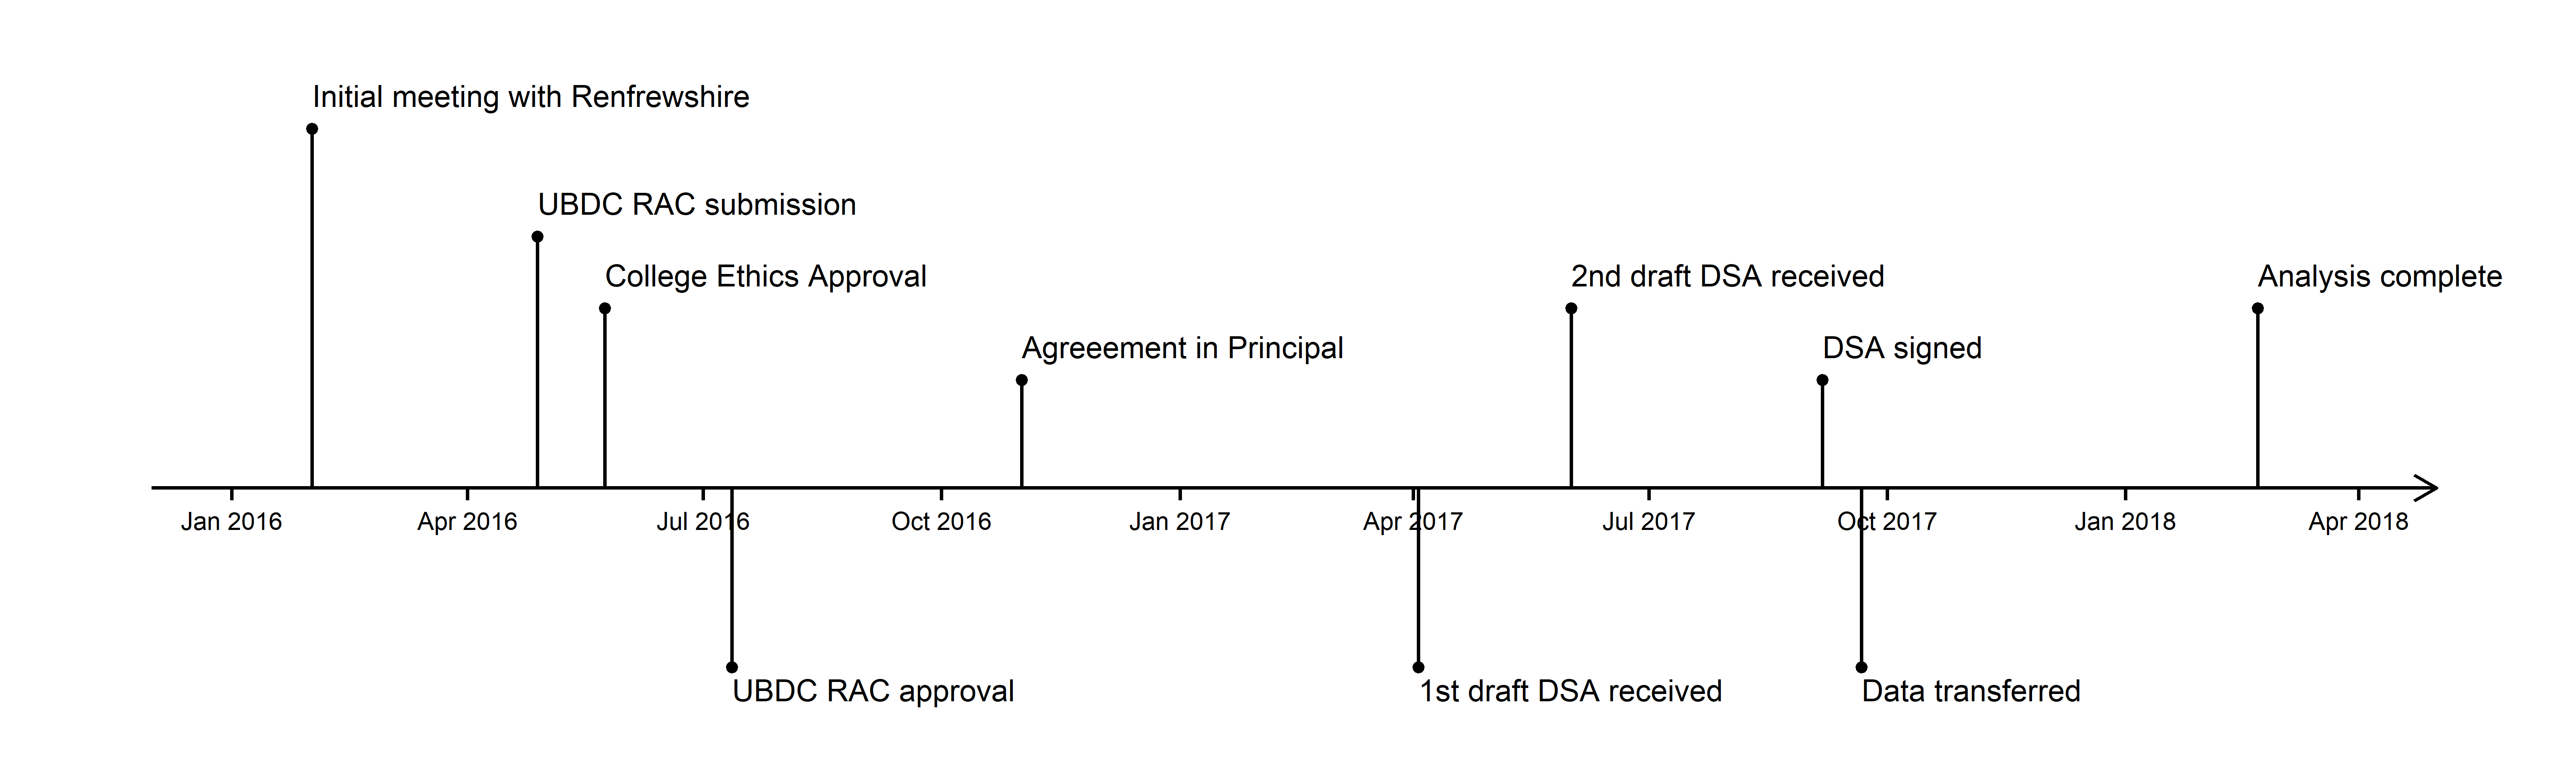
\includegraphics{figures/chapter-renf/renf-timeline.png}
    \caption{Timeline of Renfrewshire exploratory project}
    \label{fig:ren-timeline}
\end{figure}

\subsection{Data}\label{subsec:renf-methods-data}

As with all services provided by Renfrewshire council, home care data is
collected to ensure efficient management of the service and as evidence
of service provision (Renfrewshire-Council 2015). Recording of
individual episodes of care also helps with budgetary management of the
service.

For the purposes of analysis distinction is made between \emph{episodes}
and \emph{packages} of home care. An episode of care refers to each
instance a carer visits a home care client in their own home. A package
of care is the collection of repeated episodes an individual routinely
receives in a week.

Data provided for the purposes of this exploratory study included
anonymised information on; how many days per week, how many hours per
day, service provider (e.g.~local authority or independent provider),
type of care (e.g.~mainstream or reablement), start date and end date
for every episode of home care delivered to individuals in the
Renfrewshire council area between April 2006 and April 2017. Demographic
information detailing gender and year of birth was also provided.

As all episodes of home care were delivered over a period of time, data
was provided for some episodes where the care was first delivered as
early as 2004 or as late as Summer 2017 (e.g.~a home care episode
starting in December 2005 and running to December 2006 was included in
the data transfer). Data detailing information on community alarm and
telecare services provided by Renfrewshire council were not analysed as
part of this project.

Analysis focussed on individuals over the age of 65. An unexpectedly
large number of individuals (n = 112, 0.01\%) had a year of birth
recorded as 1900 (compared to n = 68 born between the years 1901 and
1910). A similar phenomenon was reported in the SCS linkage process
(described in chapter \ref{ch:methods}) with the deduction that 1900 was
a code for missing data. In this analysis these records were omitted. To
protect anonymity individual month and day of birth were not shared
meaning age was calculable from year of birth only.

The SCS requests information on the total weekly hours of home care each
individual received during the census week. To replicate this
information, every episode of care in the exploratory dataset was
summarised. For each episode of home care, the number of hours per day
was multiplied with days per week to give a weekly total of home care
hours for each episode. To identify \emph{packages} of home care,
episodes of home care with the same start and end date and of the same
home care type, were added together. For example, an individual
receiving home care of the type ``Care at Home (Mainstream)'' with an
episode of care lasting 1 hour in the morning for 3 days a week, an
episode of care lasting 45 minutes at lunchtime 7 days a week, an
evening episode of 30 minutes 7 days a week, and night-time episode of
45 mins 7 days a week, would have a total weekly home care hours count
of 17 hours per week for that home care type. Finally, the totals for
all types of home care were summed to give an overall weekly total for
each individual.

\subsection{Analysis}\label{subsec:renf-methods-analysis}

To enable analysis of the proportion of individuals captured by the
census in each year, a time-series was created for the study period 27th
March 2006 to 28th March 2016 at weekly intervals. The value of total
hours of home care each individual was receiving at each of the 523
weekly time points was identified. From this time series weekly counts
of the total number of individuals receiving home care were calculated.
Maximum and minimum values and measures of central tendency of these
weekly values were compared to the total number of individuals receiving
home care, and total number of those not captured by the census, in each
financial year.

As it was possible for individuals to receive more than one package of
care in each financial year, individuals were grouped by those that had
at least one package of care during the census week and those that had
none. This enabled comparison of the proportions of each age group,
gender, and type of home care received by whether an individual had been
identified in the census or not.

To assess the difference in the type of care received by individuals in
each of these groups, comparison was made of the total hours of home
care and total duration of care they received. Linear regression models
were fitted for the financial years 2010/11 to 2014/15 using total
weekly hours of home care or package duration (in weeks) as dependent
variables. A dummy variable indicating whether an individual had a least
one package identified in a census was used as the independent
predictor. To compare how differences in care varied across age, gender,
and care type groups, further linear models using the same parameters
were fitted to subsets of data containing these groups. This enabled
comparison of intercept and coefficient values. As the home care
packages of the types ``Community Mental Health'', ``Overnight
Services'', ``Housing Support'', and ``Extra Care Housing'' accounted
for less than one percent of packages of care, individuals receiving
these types of care were omitted from these analyses.

For individuals that received multiple packages of care, one of which
was captured by a census, the net difference in total weekly hours of
home care received across all packages was calculated in order to
summarise the variation in care. For example, an individual initially
receiving 6 hrs of care, experiencing a break in care to zero hours, and
then receiving a new package of care of 7 hrs before a further drop to 2
hrs would have a net difference of \((-6 + 7 - 5) = -4\) hours. The
distribution of this value across all individuals was then assessed.

Additional variables indicating whether home care packages were ``live''
at three, four, six, eight, and nine months before the census of each
financial year were appended to the dataset. This enabled counts of
individuals who would be captured by six-monthly, four monthly, and
three monthly census repetitions.

All data cleaning and analysis was conducted using the R language and
environment for statistical computing version 3.4.0 (R-Core-Team 2017)
with additional software packages: \texttt{dplyr} v0.7.4 (Wickham and
Francois 2017), \texttt{tidyr} v0.7.2. (Wickham and Henry 2017),
\texttt{forcats} v0.2.0 (Wickham 2017), \texttt{purrr} v0.2.4 (Henry and
Wickham 2017), \texttt{lubridate} v1.6.0. (Grolemund and Wickham 2017),
\texttt{tibbletime} v0.0.2 (Dancho and Vaughan 2017), \texttt{magrittr}
v1.5 (Bache and Wickham 2014), \texttt{broom} v0.4.2 (Robinson 2017),
\texttt{ggplot2} v2.2.1 (Wickham and Chang 2016), and \texttt{ggthemes}
v3.5.0 (Arnold et al. 2018) via the Integrated Development Environment
RStudio v1.0.143 (RStudio-team 2016). Data was held securely in the safe
haven environment described in section \ref{subsec:safe-haven}

\FloatBarrier

\section{Results}\label{sec:renf-results}

\subsection{Descriptive statistics}\label{subsec:renf-descriptives}

\textbf{re-write this paragraph describing the time series in a better
fashion - also re-check the numbers I don;t think these take account of
reinclusion of mental health etc. packages}

After data cleaning, information on 41,002 packages of home care
received by 10,130 individuals during the period 2006 to 2016 were
included in the analysis. The number of records retained at each stage
of the cleaning process is shown in table \ref{tab:renf-cleaning}. Of
these packages, 28,775 described actual packages of care. The remainder
described place holders for each individual where they were not
receiving care, either because of a break in care or because care
provision had ended altogether. These 12,227 records showed a value of
zero for the total hours of homecare received and in the case of care
provision having ended, showed an end date of 28th March 2016.

\begin{table}[h]
\centering
\begin{threeparttable}
\begin{tabular}{@{}lr@{}}
\toprule
Data Cleaning stage                & Number of records \\ \midrule
Initial home care file             & 106,111           \\
Including over 65s only            & 92,723             \\
Summarised to packages of care     & 41,002\tnote{1}    \\ 
Packages of non-zero hours of care & 28,775             \\ \bottomrule
\end{tabular}
\begin{tablenotes}
\item[1] Total number of individuals = 10,310
\end{tablenotes}
\end{threeparttable}
\caption{Number of records at each stage of data cleaning}
\label{tab:renf-cleaning}
\end{table}

Mean age of those included in the analysis was 80.8 years and median age
was 81. Sixty-four percent of individuals (n = 6,515) were female.
Detailed breakdown of age and gender groups is shown in figure
\ref{fig:ren-age-gen}. The highest absolute numbers of individuals are
found in the 76-85 age group. Statistical disclosure control meant that
grouping an additional age group for over 95s was not possible.

\begin{figure}[]
  \centering
    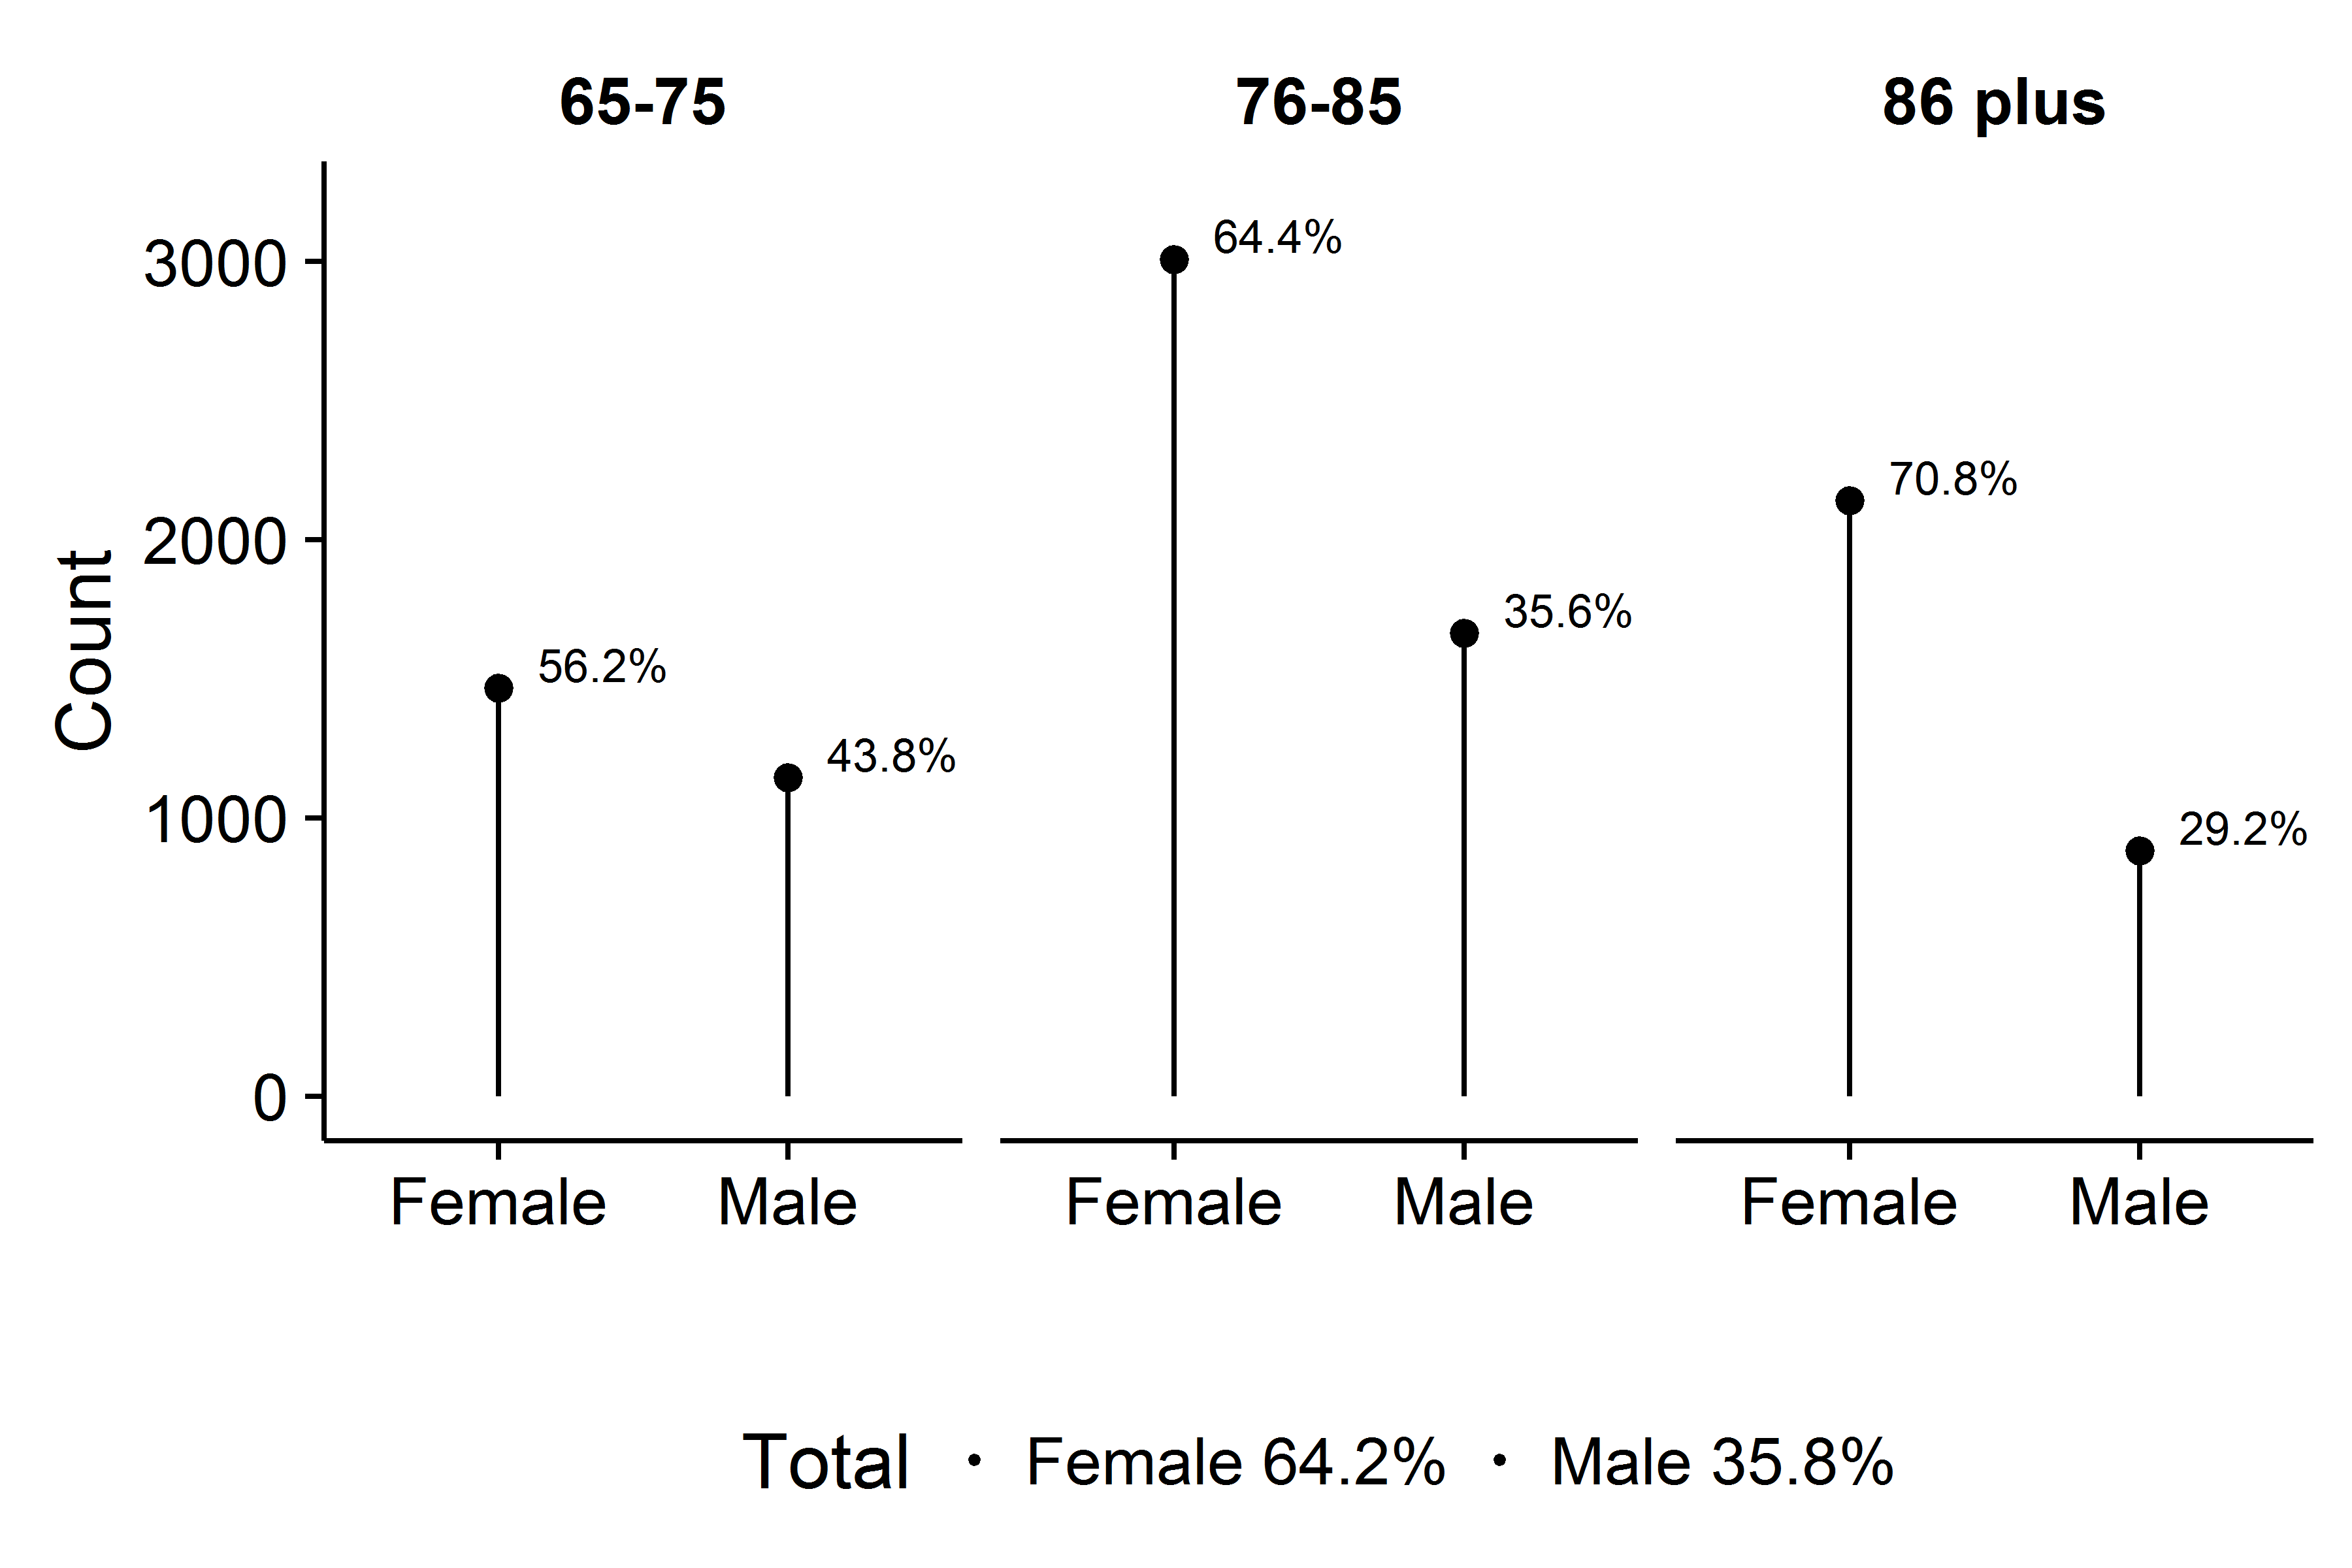
\includegraphics[height = 10cm]{figures/chapter-renf/01-age-gender-ts-subset.png}
    \caption{Count and proportion of indidividuals receiving home care by age and gender}
    \label{fig:ren-age-gen}
\end{figure}

Seventy-eight percent of home care packages (n=22,484) were provided for
``Care at Home (Mainstream)'' with ``Reablement'' type packages making
up the majority of the remainder (Figure \ref{fig:ren-type}). Only 60
packages of care for over 65s were classified as being provided for
``Community Mental Health'' or ``Overnight Services'' during the study
period. ``Reablement'' packages were first coded as such in the
financial year 2010/11 meaning ``Care at Home (Mainstream)'' made up an
even larger proportion of care packages prior to this.

\begin{figure}[]
  \centering
    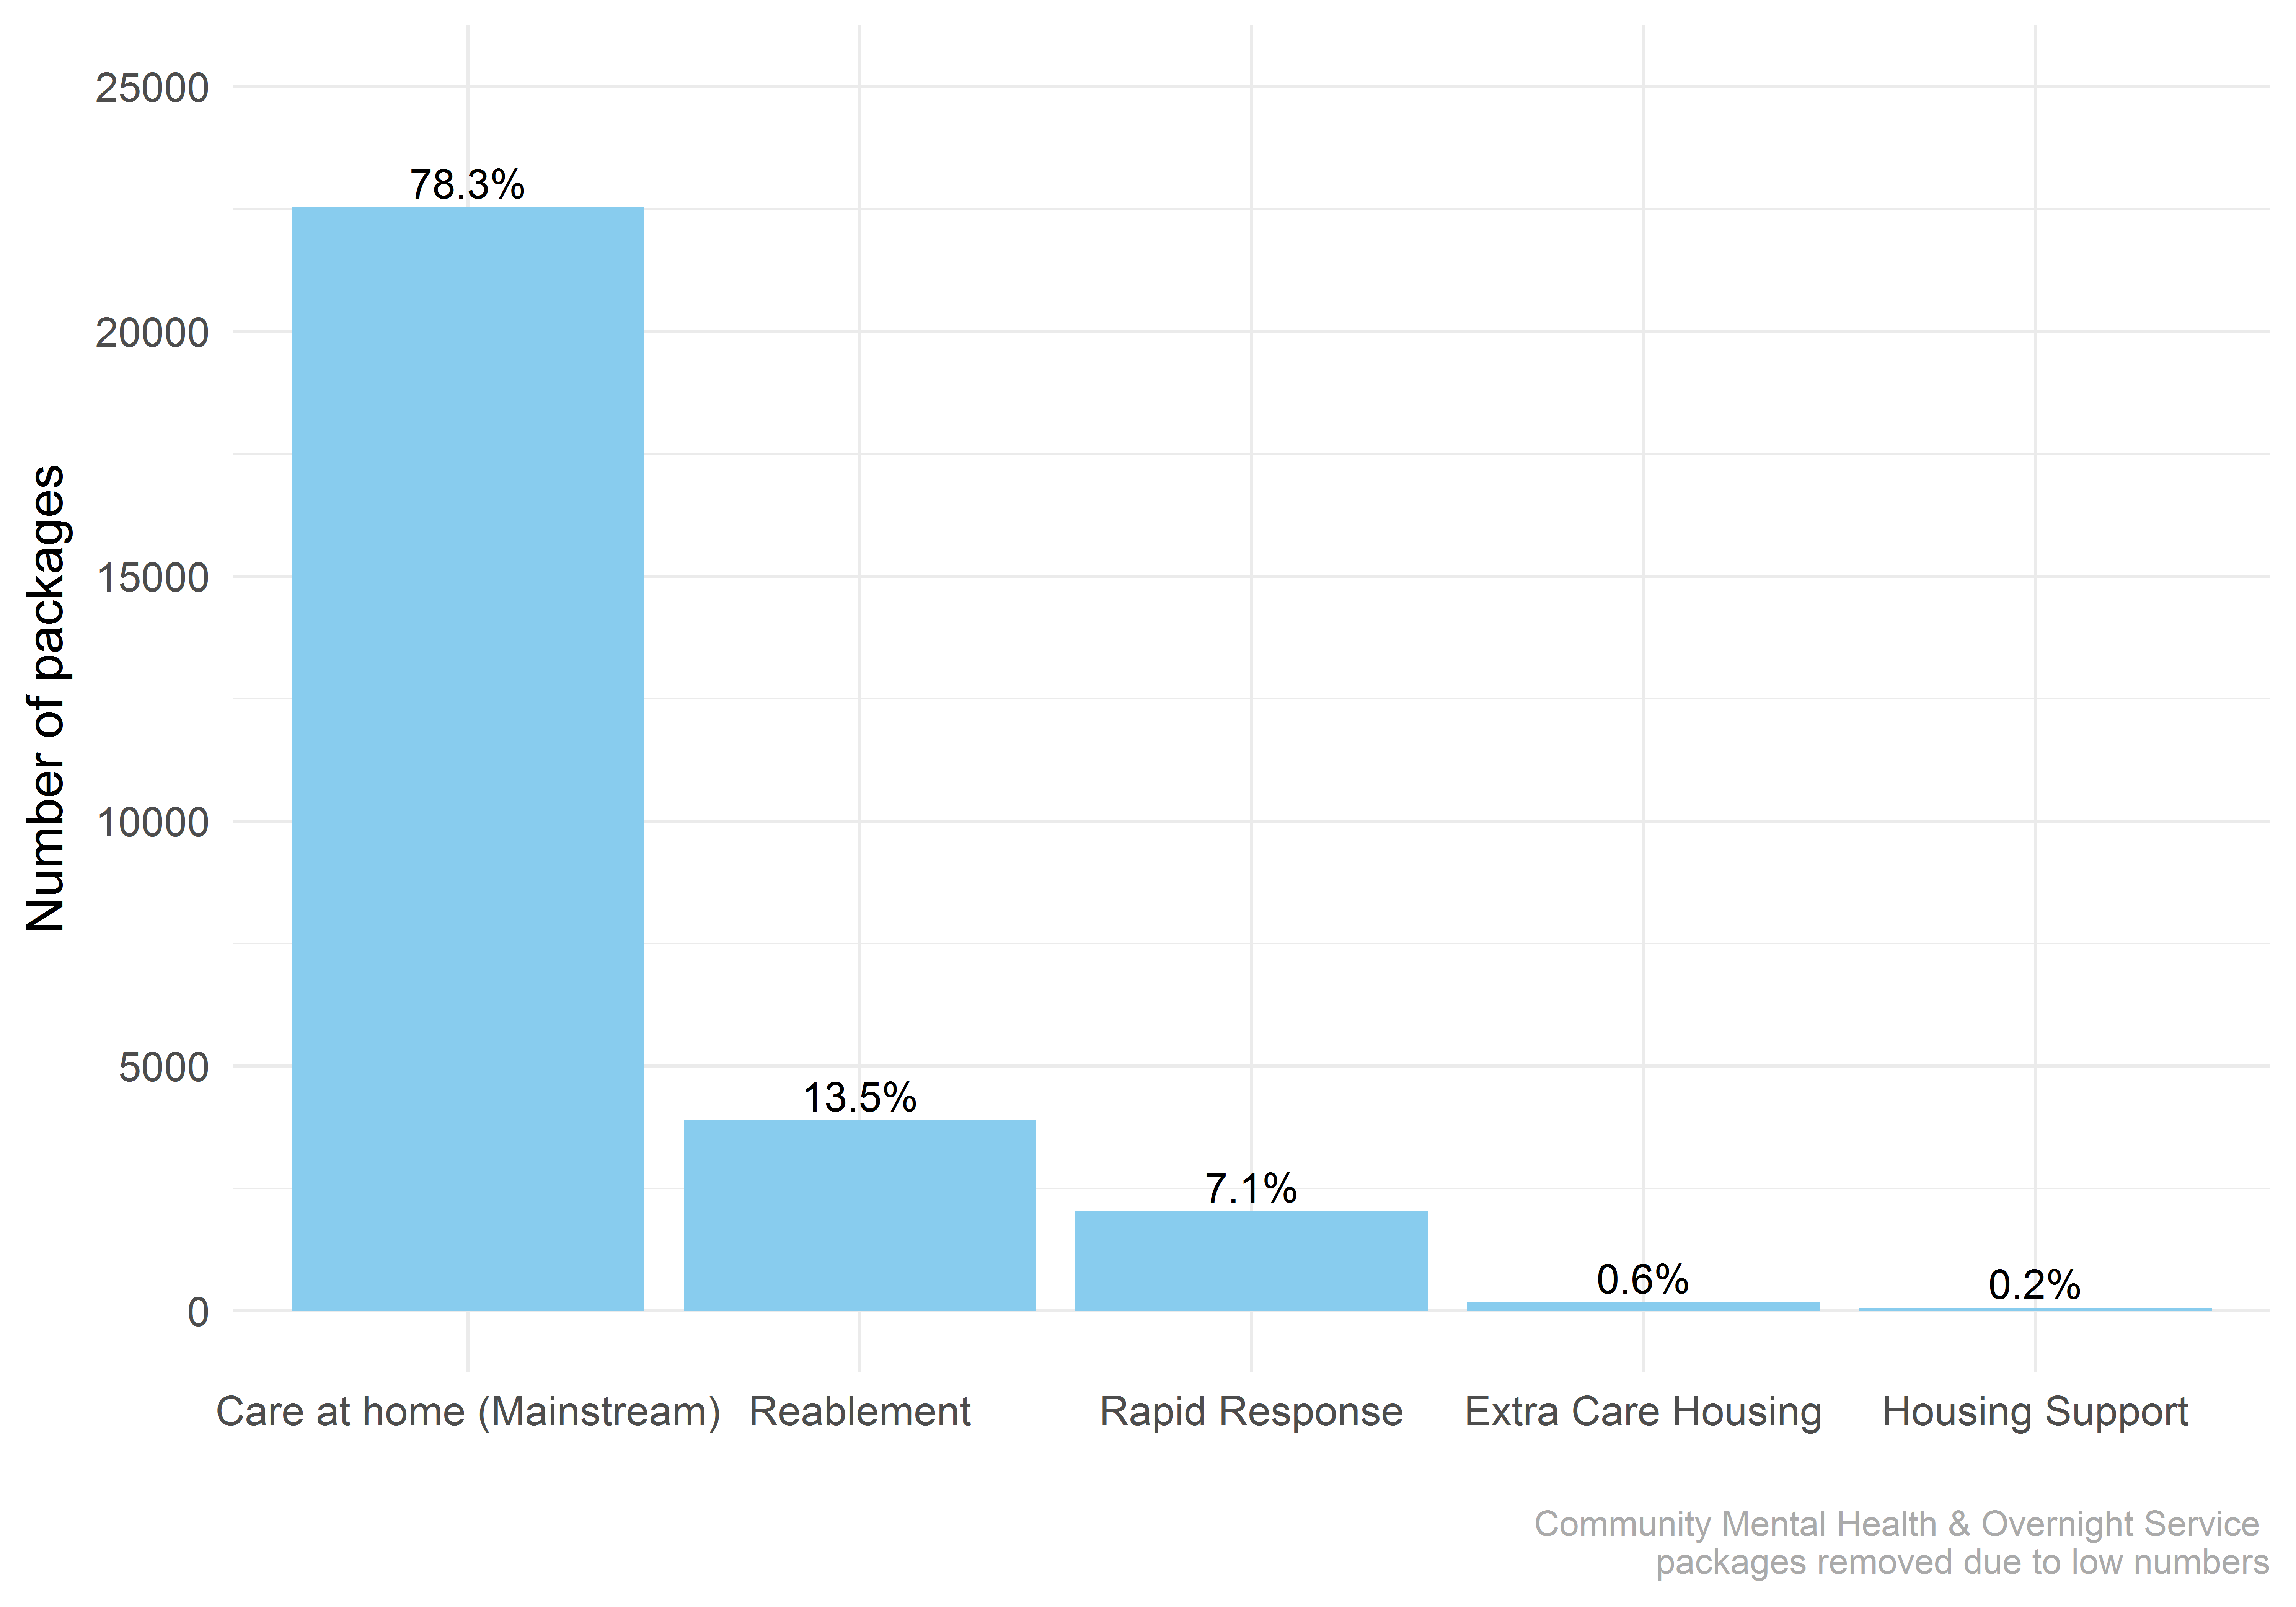
\includegraphics[height = 10cm]{figures/chapter-renf/03-pack-plot}
    \caption{Count and proportion of home care type}
    \label{fig:ren-type}
\end{figure}

Almost two-thirds of home care packages in the study period provided
care at intensities of less than 10 hours per week. Only 1,352 (4.7\%)
packages over the 10 year study period provided high intensity care of
over 20 hours per week (figure \ref{fig:ren-hrs}). Eighty-five percent
of packages lasted for less than one year (figure
\ref{fig:ren-duration}).

\begin{figure}[]
  \centering
    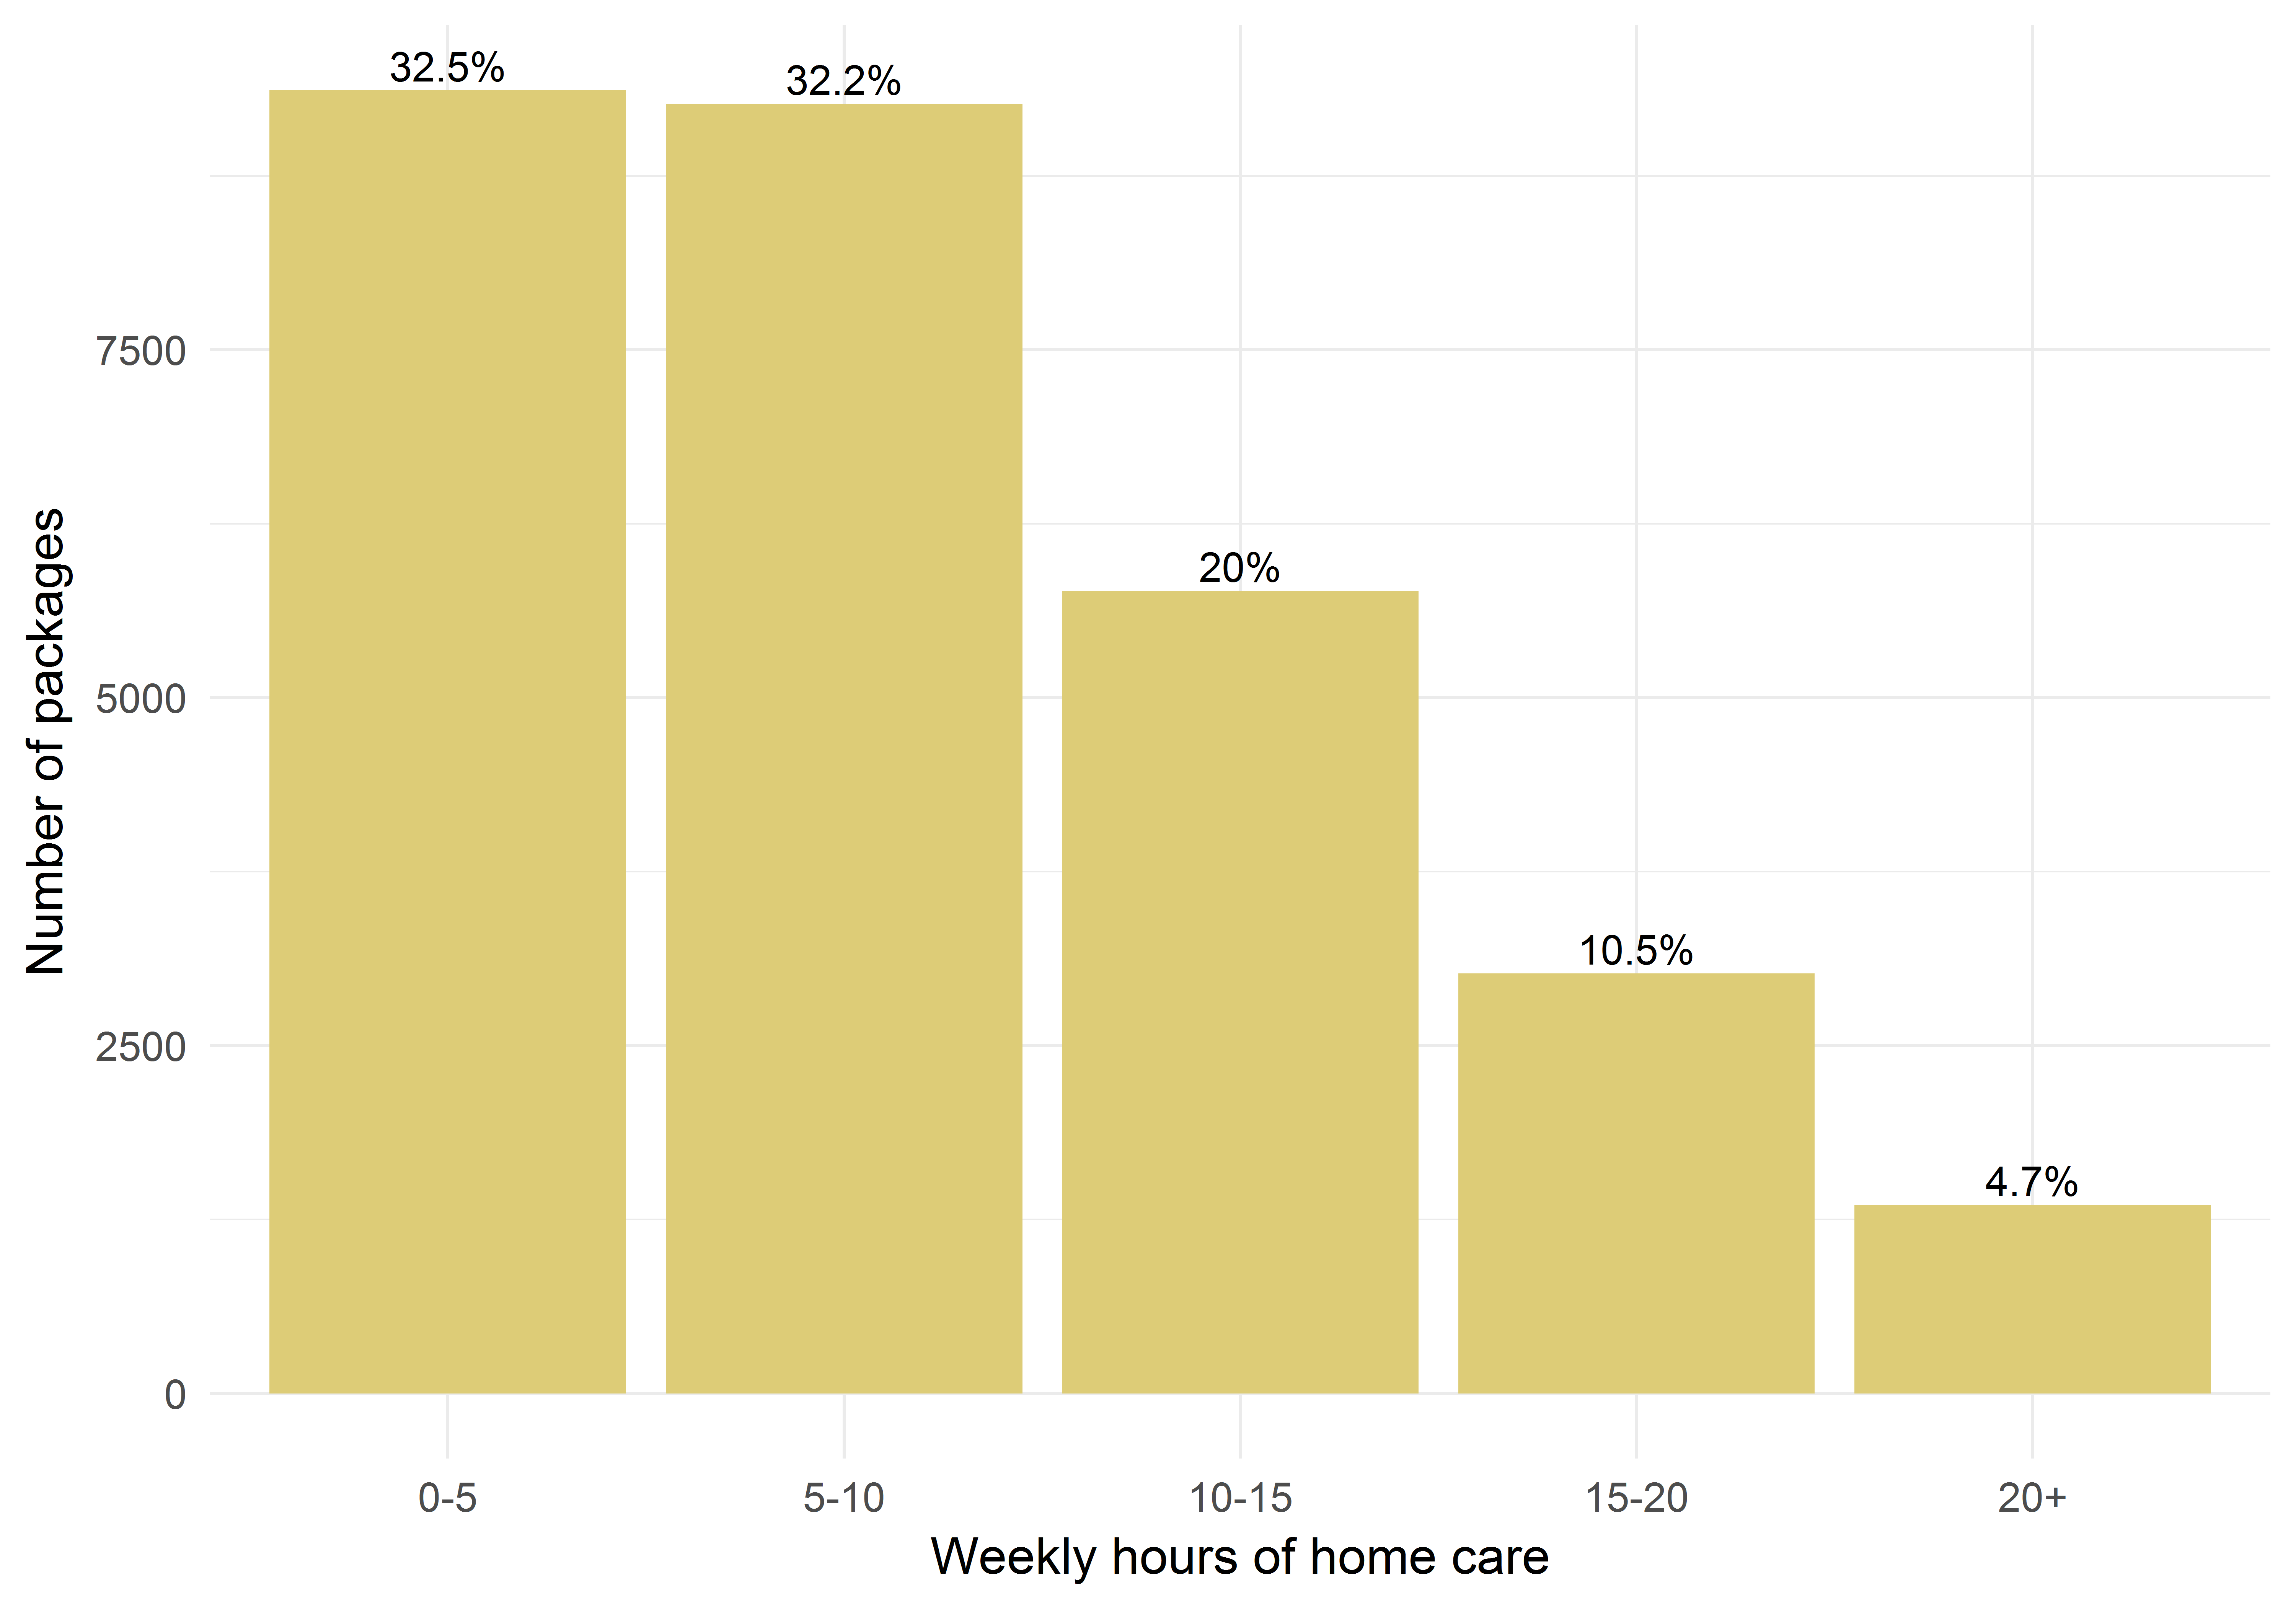
\includegraphics[height = 10cm]{figures/chapter-renf/04-hrs-plot-ts-subset.png}
    \caption{Count of packages of care by intensity}
    \label{fig:ren-hrs}
\end{figure}

\begin{figure}[]
  \centering
    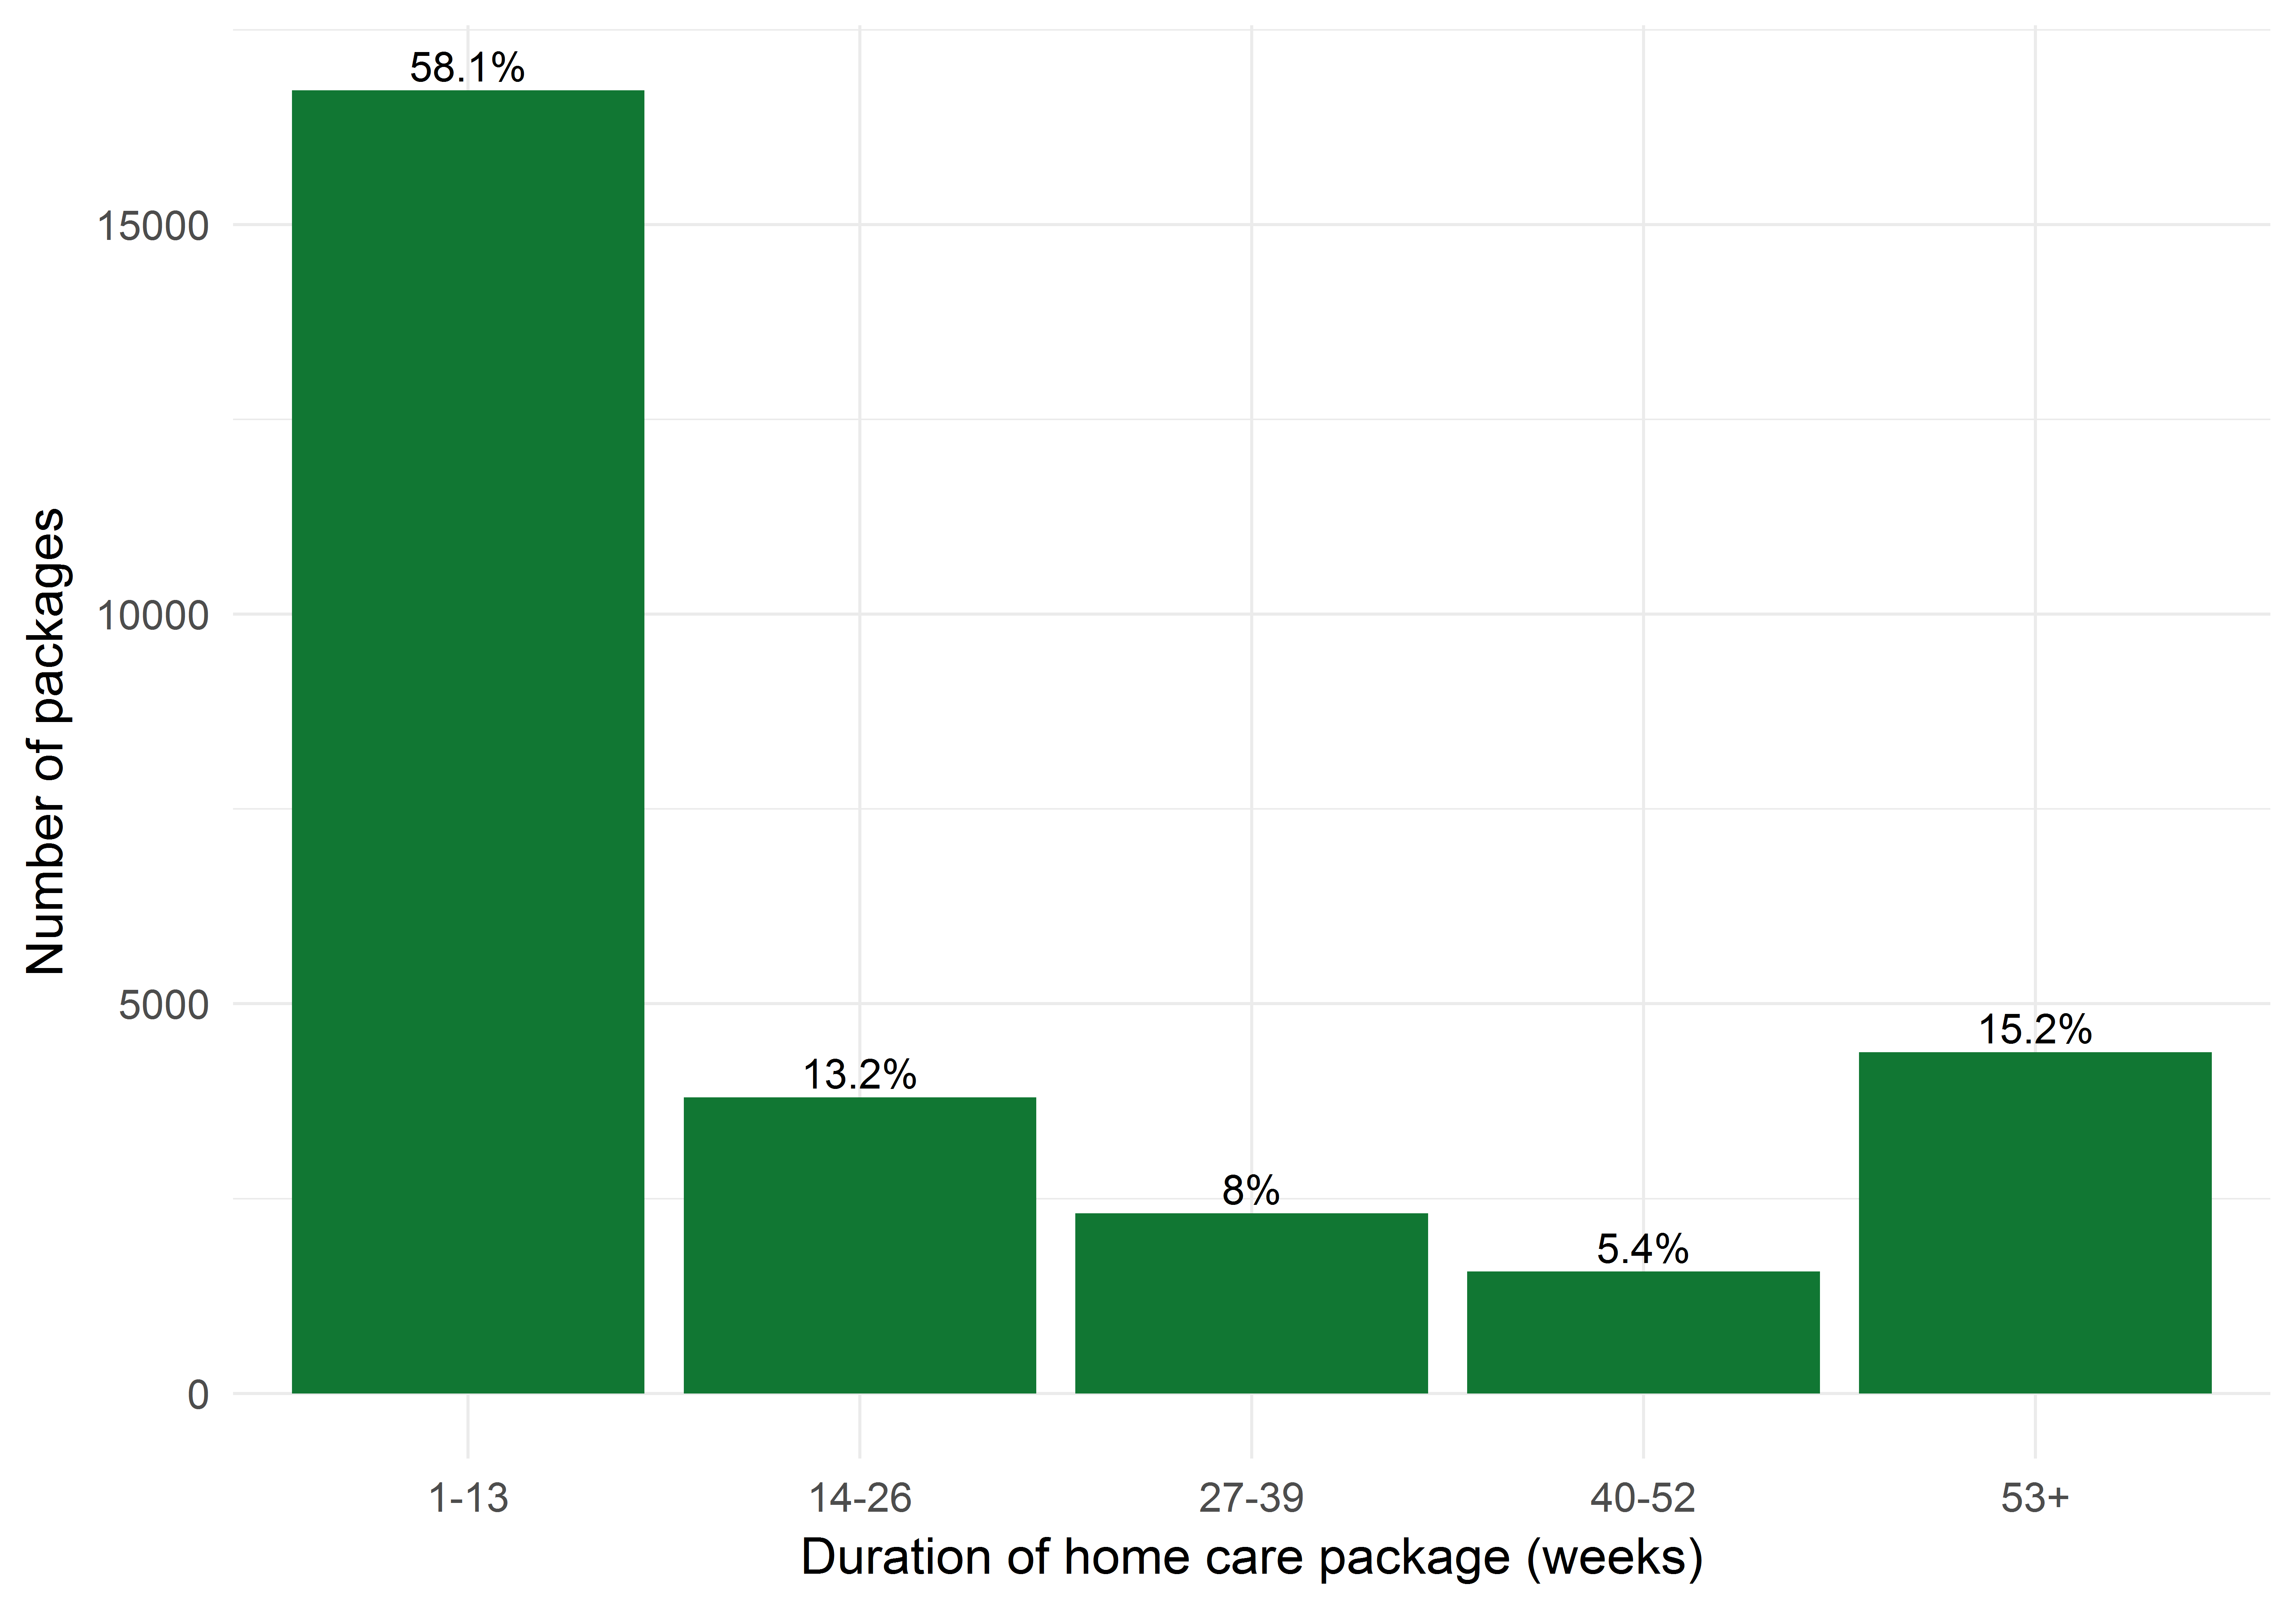
\includegraphics[height = 10cm]{figures/chapter-renf/05-duration-plot.png}
    \caption{Count of packages of care by duration}
    \label{fig:ren-duration}
\end{figure}

\FloatBarrier

\subsection{Distribution of individuals receiving home care}\label{renf-results-ts}

Table \ref{tab:renf-ts-summary} and figure \ref{fig:renf-hrs} show the
variation in the number of people receiving home care during each
financial year. There is little weekly variation within years with the
exception of financial year 2010/11 which saw a large drop in the total
number of individuals receiving care. The variation in years following
this show gradual increases and overall numbers return to pre-2010/11
levels by 2014/15.

\begin{figure}[h]
  \centering
    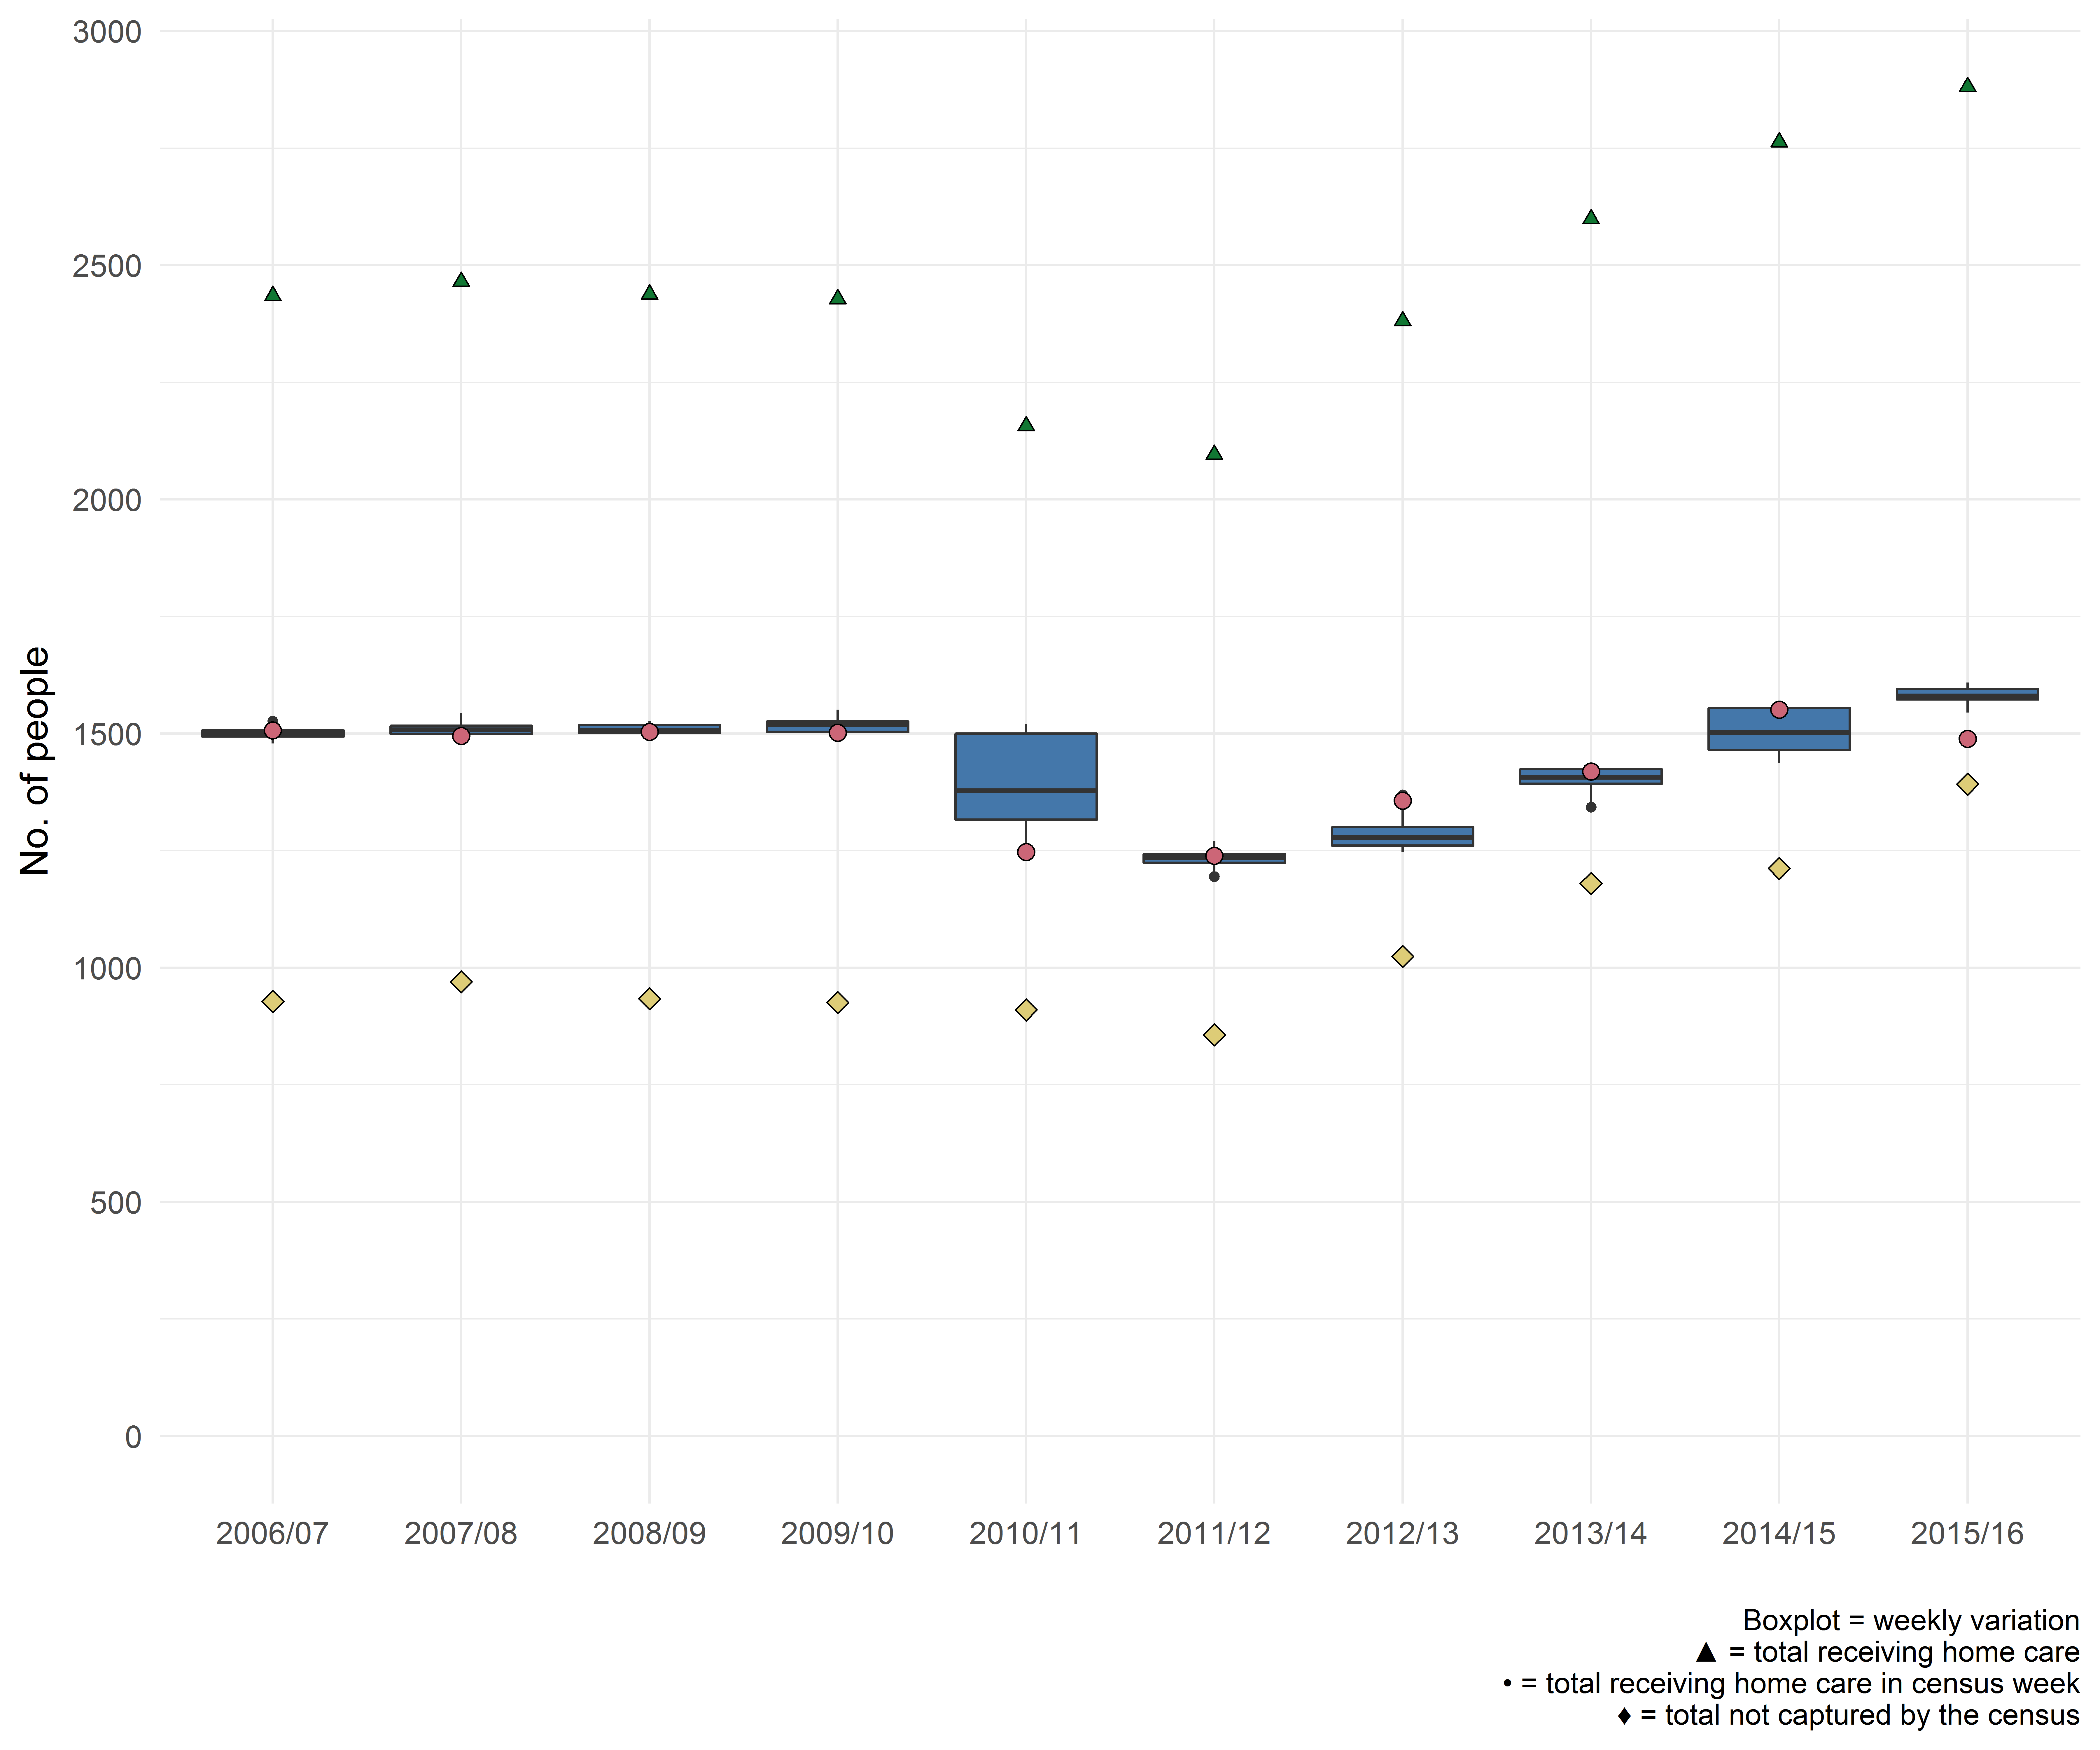
\includegraphics{figures/chapter-renf/06-individual-weekly-variation.png}
    \caption{Variation in the number of individuals receiving home care}
    \label{fig:renf-hrs}
\end{figure}

Figure \ref{fig:renf-hrs} and table \ref{tab:renf-ts-summary} also
indicate that number of individuals receiving home care and captured by
the census is between 51.7\% and 61.9\% of the total number of
individuals that will receive care in that year. The trend shows a
decreasing proportion of individuals are captured by the census.

\begin{table}[]
\centering
\resizebox{\textwidth}{!}{%
\begin{tabular}{@{}lrrrrrrrrrr@{}}
\toprule
\textbf{\begin{tabular}[c]{@{}l@{}}Financial\\ Year\end{tabular}} & \textbf{min} & \textbf{max} & \textbf{mean} & \textbf{sd} & \textbf{median} & \textbf{range} & \textbf{IQR} & \textbf{\begin{tabular}[c]{@{}r@{}}Total individuals\\ receiving home\\ care\end{tabular}} & \textbf{\begin{tabular}[c]{@{}r@{}}Total individuals\\ not captured by\\ census\end{tabular}} & \textbf{\begin{tabular}[c]{@{}r@{}}Ratio of individuals\\ captured by census\\ (\%)\end{tabular}} \\ \midrule
\textbf{2006/07} & 1479 & 1527 & 1502.51 & 11.75 & 1501 & 48 & 15 & 2435 & 928 & 61.89 \\
\textbf{2007/08} & 1488 & 1544 & 1508.65 & 12.61 & 1508 & 56 & 18 & 2465 & 970 & 60.65 \\
\textbf{2008/09} & 1486 & 1527 & 1508.63 & 9.96 & 1508 & 41 & 16 & 2438 & 934 & 61.69 \\
\textbf{2009/10} & 1488 & 1551 & 1516.43 & 15.62 & 1520 & 63 & 24 & 2428 & 926 & 61.86 \\
\textbf{2010/11} & 1256 & 1520 & 1399.39 & 90.85 & 1378 & 264 & 176 & 2157 & 910 & 57.81 \\
\textbf{2011/12} & 1195 & 1271 & 1234.19 & 15.21 & 1236 & 76 & 19 & 2096 & 857 & 59.11 \\
\textbf{2012/13} & 1248 & 1369 & 1288.44 & 36.55 & 1278 & 121 & 39 & 2381 & 1024 & 56.99 \\
\textbf{2013/14} & 1343 & 1436 & 1405.52 & 21.17 & 1408 & 93 & 31 & 2599 & 1180 & 54.60 \\
\textbf{2014/15} & 1437 & 1568 & 1505.50 & 44.68 & 1502 & 131 & 90 & 2763 & 1212 & 56.13 \\
\textbf{2015/16} & 1545 & 1609 & 1582.60 & 13.27 & 1580 & 64 & 21 & 2881 & 1392 & 51.68 \\ \bottomrule
\end{tabular}%
}
\caption{Variation in the number of individuals receiving home care}
\label{tab:renf-ts-summary}
\end{table}

\FloatBarrier
\subsection{Comparison of individuals with/without any packages in the census}\label{subsec:renf-pack-diff}

Table \ref{tab:renf-cens-indi-count} shows the number of individuals
with at least one package captured by the census compared to those that
have zero packages during the census week in each financial year. There
is very little variation in the proportions in each group over time.
\textbf{This needs to be a table showing the number of indiviudals with
only one package of care in the year and the number with multiple
packages and should be in section 4.4.6}

\begin{table}[]
\centering
\begin{tabular}{@{}lrr@{}}
\toprule
\textbf{Financial Year} & \textbf{\begin{tabular}[c]{@{}r@{}}Individuals with zero\\ packages captured by \\ census (n)\end{tabular}} & \textbf{\begin{tabular}[c]{@{}r@{}}Individuals with at\\ least one package \\ captured by census (n)\end{tabular}} \\ \midrule
\textbf{2010/11} & 864 (40.3\%) & 1279 (59.7\%) \\
\textbf{2011/12} & 797 (38.2\%) & 1289 (61.8\%) \\
\textbf{2012/13} & 945 (39.8\%) & 1430 (60.2\%) \\
\textbf{2013/14} & 1080 (41.7\%) & 1513 (58.3\%) \\
\textbf{2014/15} & 1138 (41.4\%) & 1614 (58.6\%) \\ \bottomrule
\end{tabular}
\caption{Count of individuals with packages captured by census}
\label{tab:renf-cens-indi-count}
\end{table}

As shown in figure \ref{fig:renf-prop-plot-age}, there is very little
difference in age and gender groups between those that are not captured
by the census in each year compared to those that are represented in the
census.

\begin{figure}[]
  \centering
    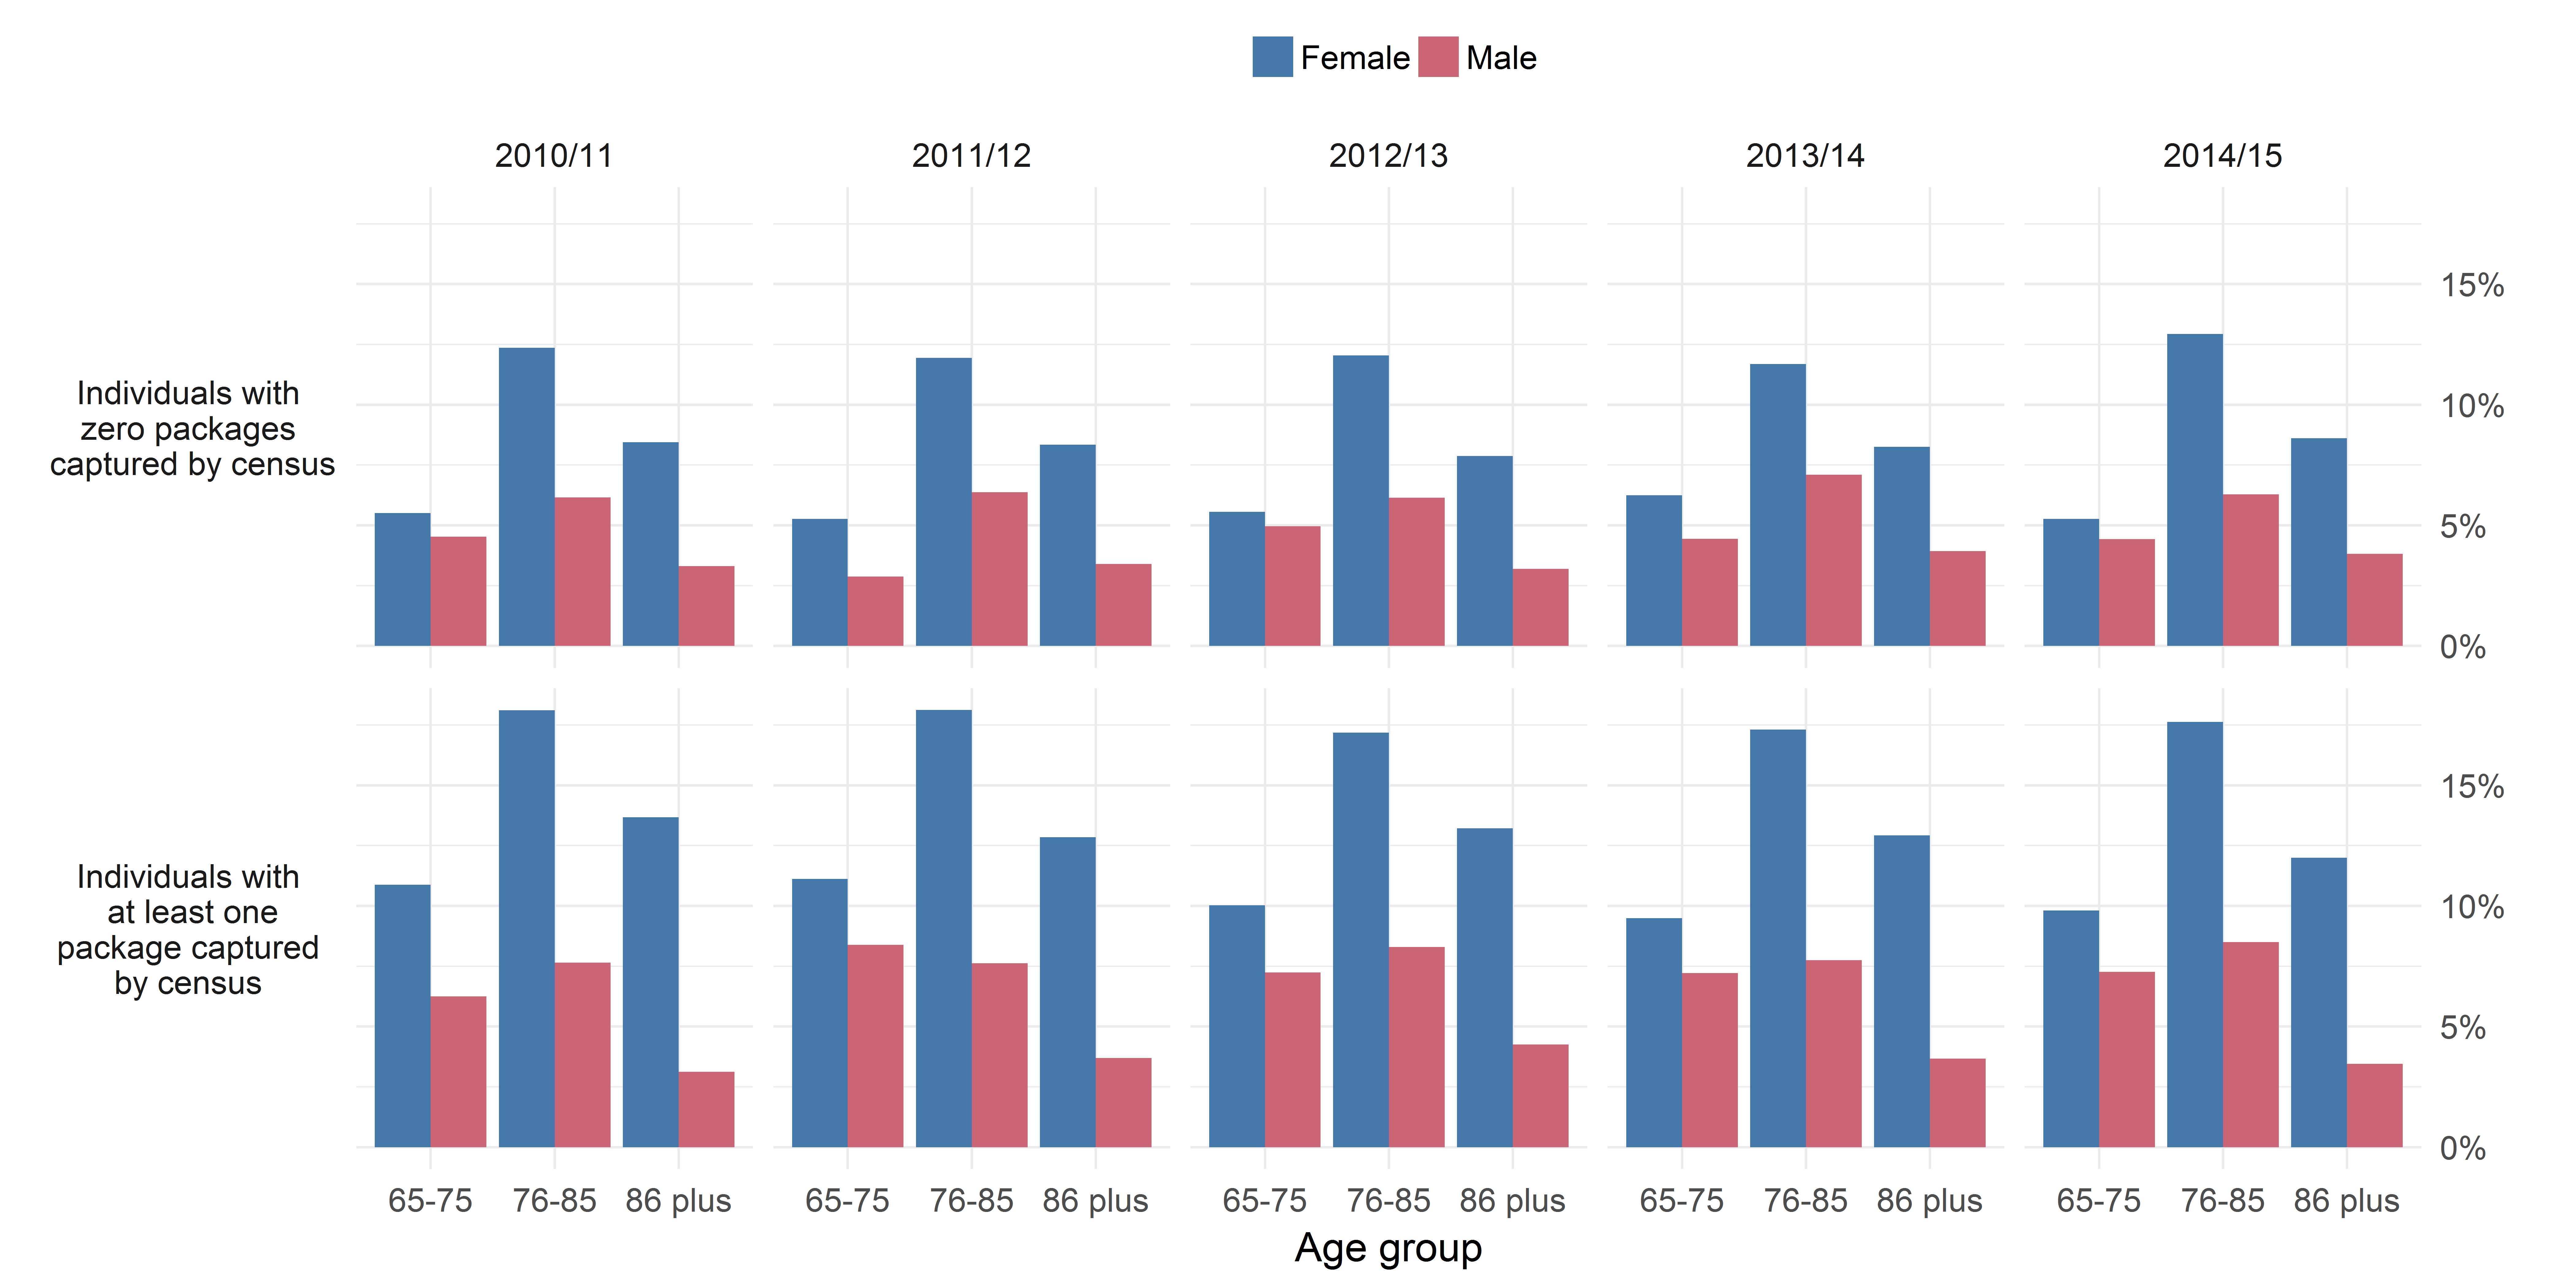
\includegraphics{figures/chapter-renf/12a-prop-plot-age.png}
    \caption{Proportion of individuals receiving home care}
    \label{fig:renf-prop-plot-age}
\end{figure}

Figure \ref{fig:renf-prop-plot} shows that there are similar proportions
of individuals receiving each type of homecare in each financial year
regardless of whether or not they have any packages of care captured by
the census. The figure also shows the increasing proportion of
``Reablement'' packages over time from almost no packages in 2010/11 to
approximately 14\% of all packages delivered in 2014/15. ``Care at home
(Mainstream)'' type packages saw a drop from approximately 82\% to 60\%
of all packages over the same period.

\begin{figure}[]
  \centering
    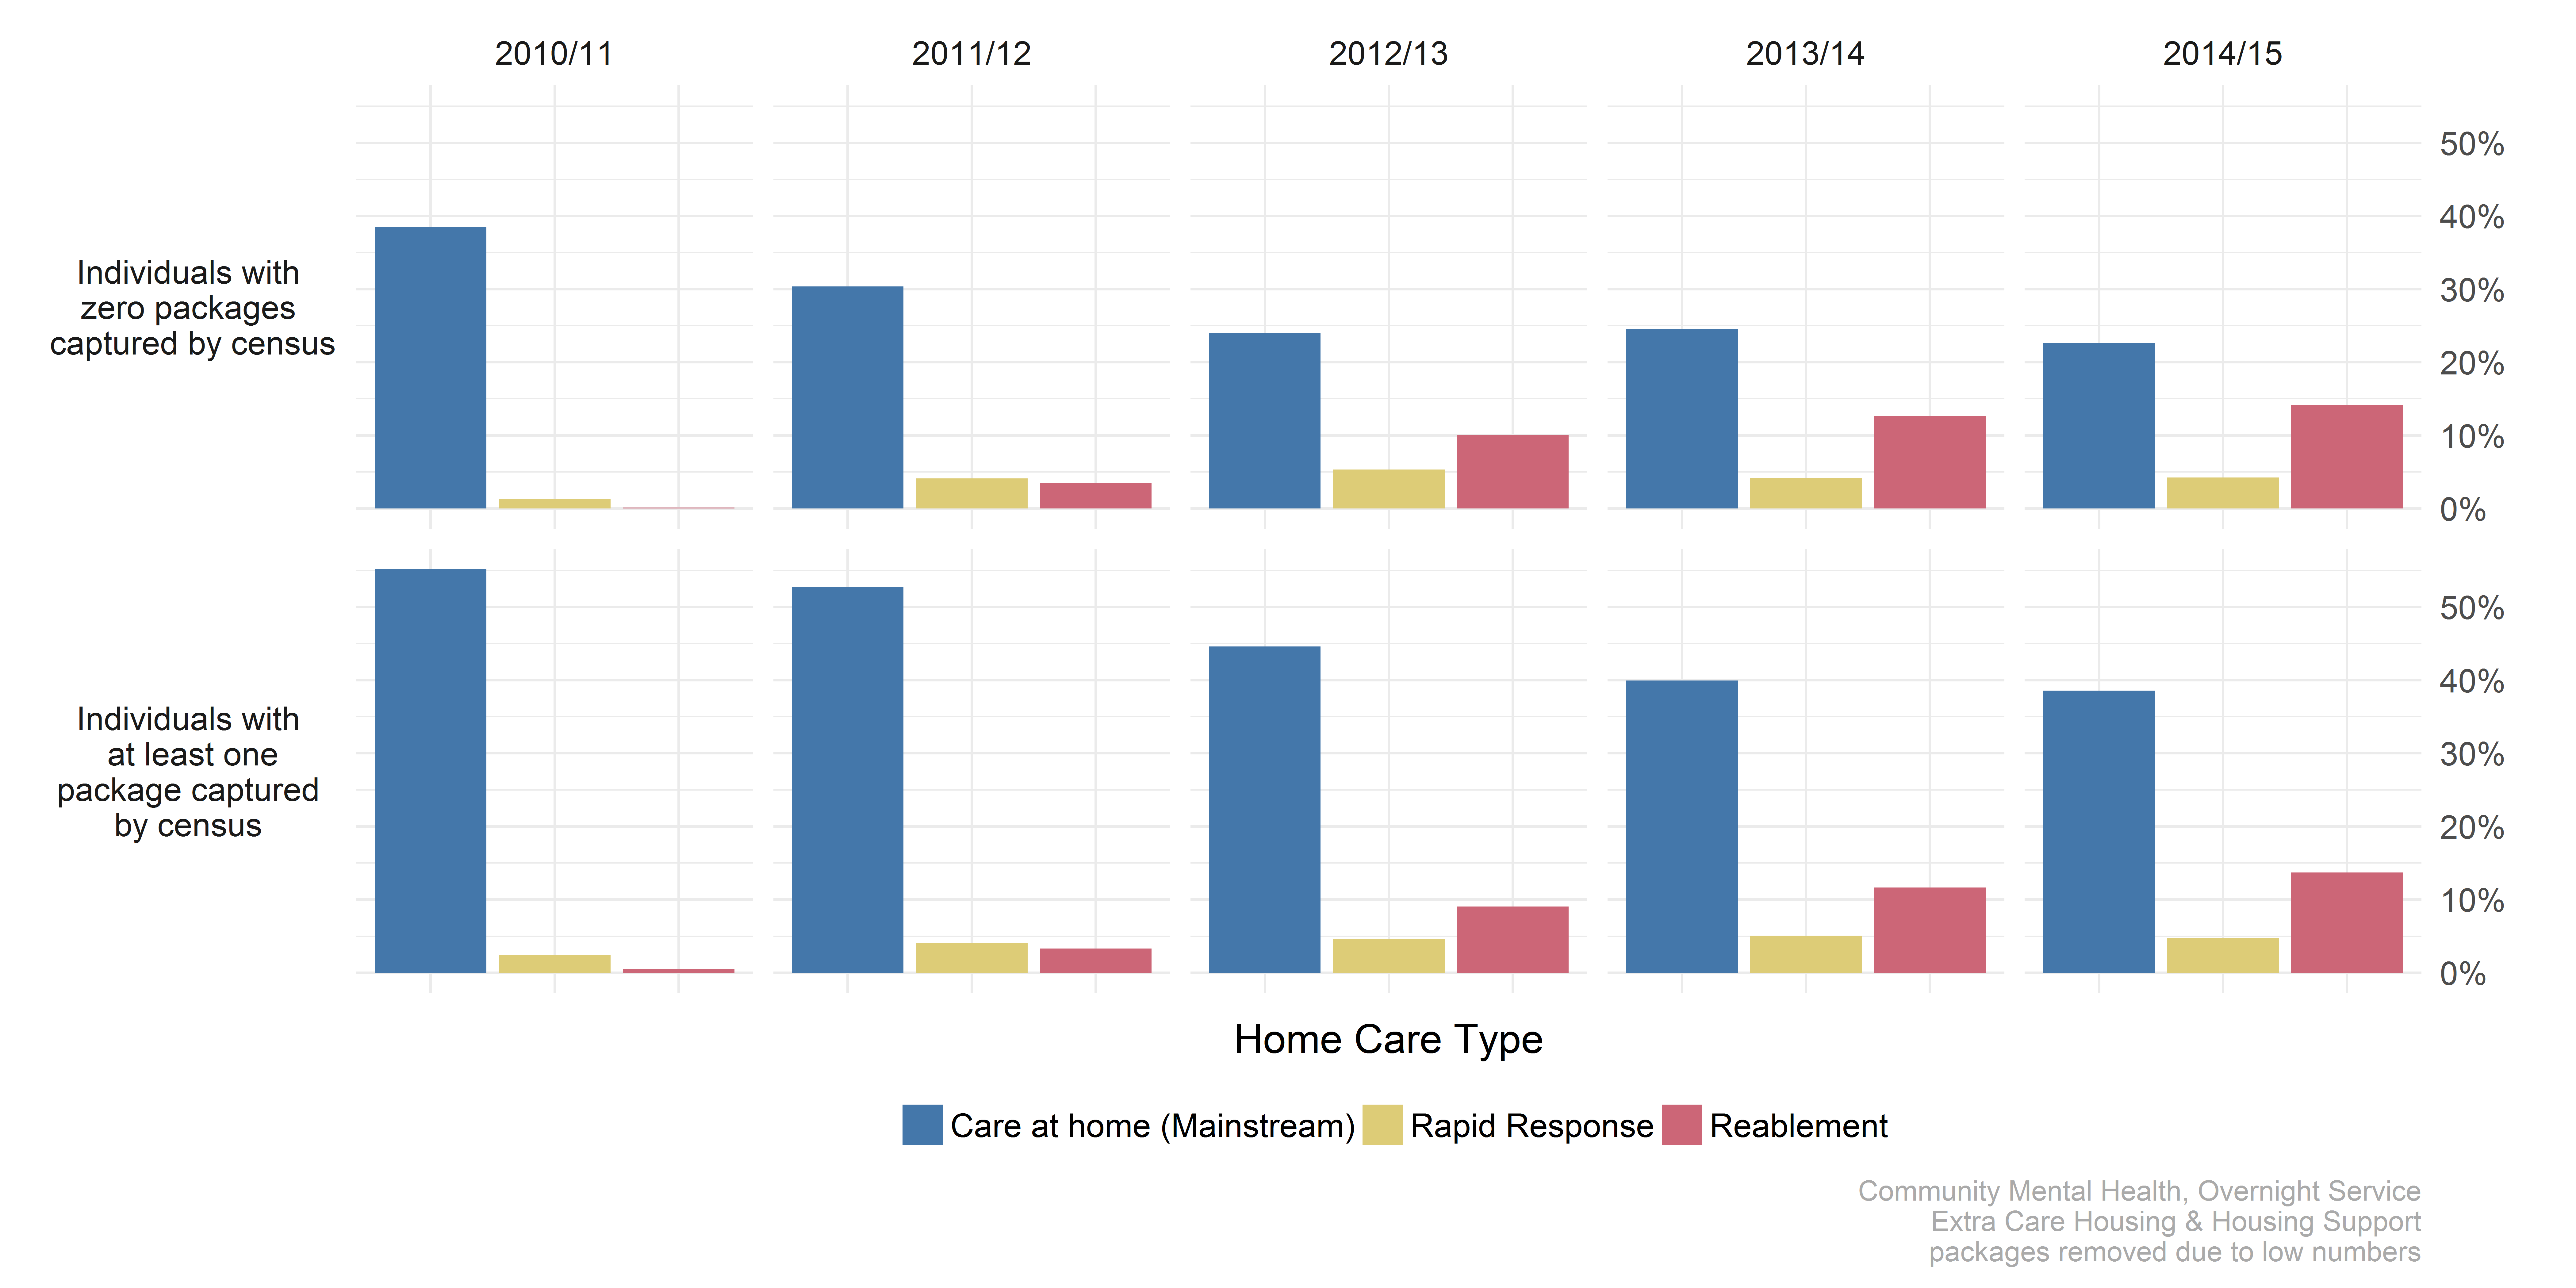
\includegraphics{figures/chapter-renf/12c-census-prop-plot.png}
    \caption{Proportion of individuals receiving home care}
    \label{fig:renf-prop-plot}
\end{figure}

\FloatBarrier

\subsection{Comparison of package intensity for individuals with/without any packages in the census}\label{subsec:renf-inten-diff}

Comparison of the total weekly hours of home care (intensity) that
individuals with/without any packages in the census receive (figure
\ref{fig:renf-inten}) shows that there is very little difference in
median values. However, as time progresses, the median value for total
hours of home care is slightly larger for those with no packages of care
captured in the census.

This trend is shown in table \ref{tab:renf-regr-inten} which shows the
intercept and coefficient of total hours of home care in linear
regression models for each year (in bold) with presence of at least one,
or zero packages in the census as a categorical predictor. Over time,
the intercept value increases from 6.26 hours in 2010/11 to 8.41 hrs in
2014/15 indicating a general increase in intensity for individuals with
at least one package in the census. There is a statistically significant
difference in the amount of hours of care received between those that
have at lease one package in the census and those that have no packages
in every financial year. The coefficient value is negative in 2010/11
but positive in all other years and increases over time. However, the
difference in groups is modest (the 1.2 hrs increase in intensity in
2014/15 is equivalent to approximately 10 minutes extra care per day).

\begin{figure}[h]
  \centering
    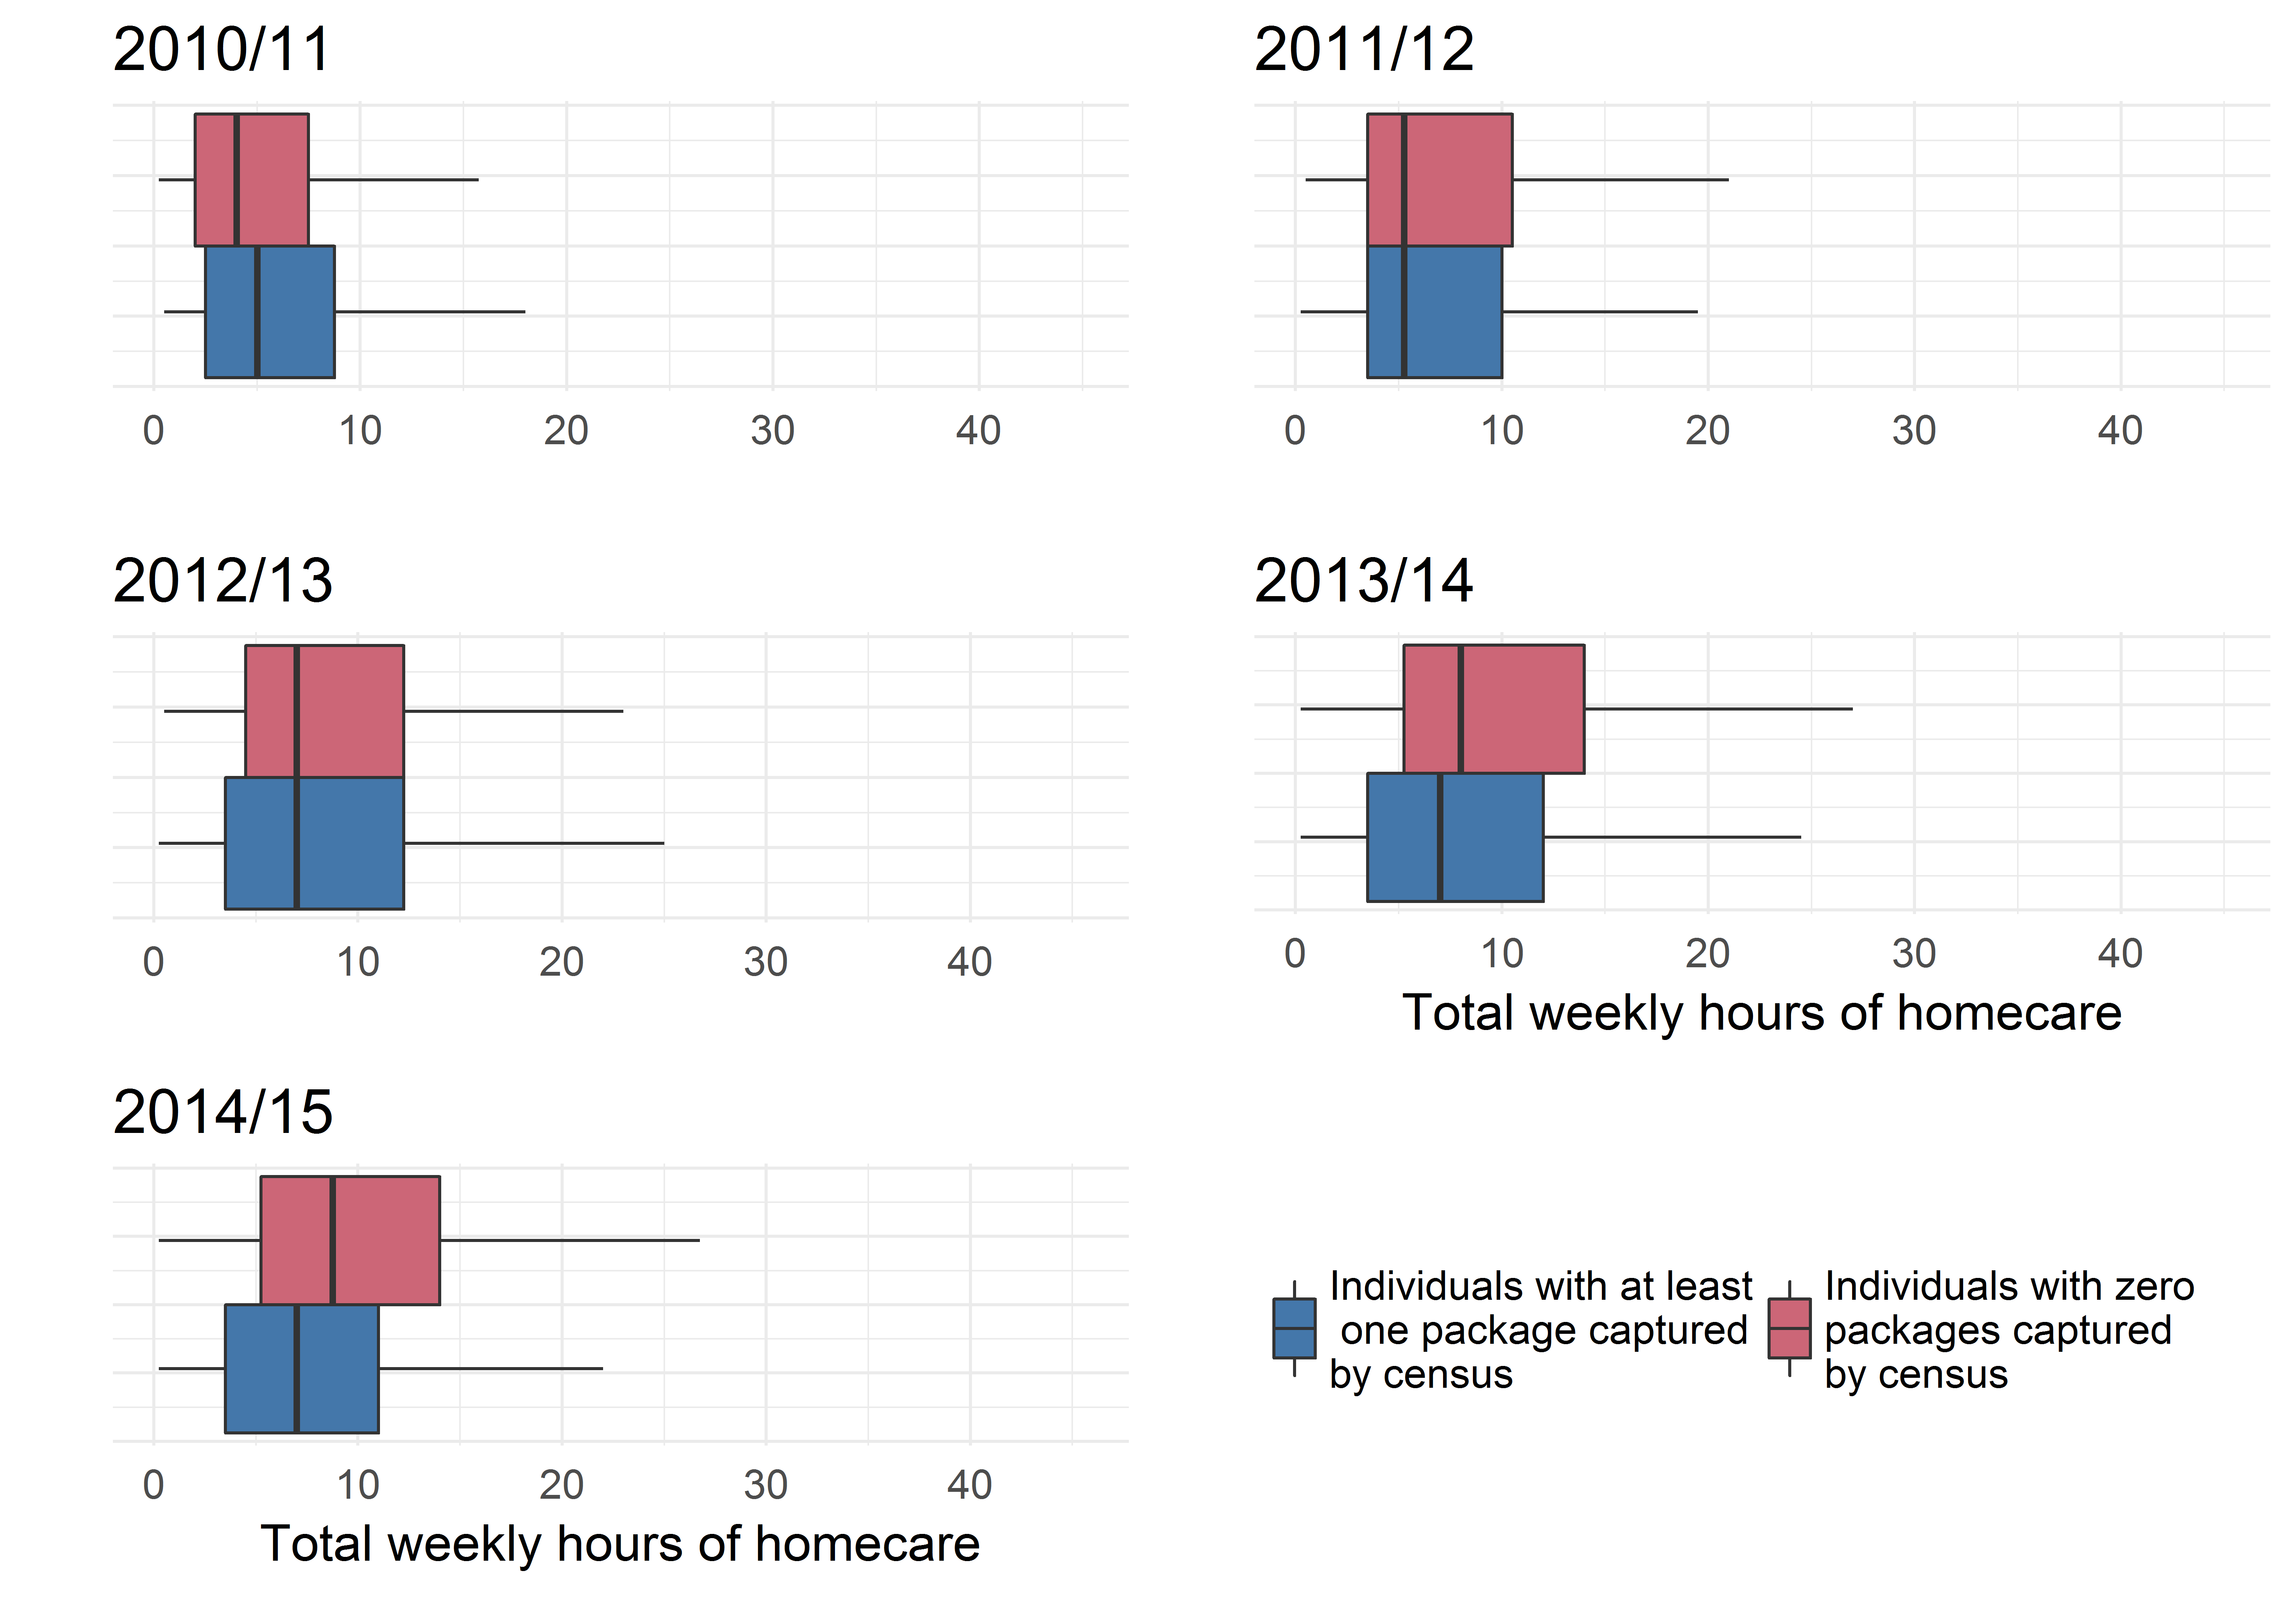
\includegraphics{figures/chapter-renf/14-inten.png}
    \caption{Variation in intensity of home care}
    {\scriptsize outlying points removed to avoid disclosure}
    \label{fig:renf-inten}
\end{figure}

Table \ref{tab:renf-regr-inten} also shows the results of the same
linear regression model applied separately to individuals from groups of
different gender, age, and home care type. The differences between
theses groups become more apparent over time with all groups (apart from
the ``Rapid Response'' care type) showing statistically significant
differences in 2014/15. Intercept values for total hours of home care
vary slightly across different groups with ``Rapid Response'' and
``Reablement'' packages more likely to have higher values - particularly
in later years. Differences between groups also vary with older age
groups and ``Reablement'' care type packages showing larger coefficient
values for those with zero packages captured by the census. The largest
difference is seen for ``Reablement'' packages in 2014/15 with an
expected 2.14 hrs increase for those with zero packages compared to
those with at least one package in the census. This is equivalent to an
18.3 minute increase in care per day. The variation in total hours of
care between home care types is plotted in figure
\ref{fig:renf-intensity-type}.

\begin{landscape}
\begin{longtable}[c]{@{}lllllllll@{}}
\caption{Regression models of package intensity}
\label{tab:renf-regr-inten}\\
\toprule
\textbf{\begin{tabular}[c]{@{}l@{}}Financial\\ Year\end{tabular}} & \textbf{Gender} & \textbf{Age group} & \textbf{Type of home care} & \textbf{} & \textbf{estimate} & \textbf{std.error} & \textbf{statistic} & \textbf{p value} \\* \midrule
\endfirsthead
%
\multicolumn{9}{c}%
{{\bfseries Table \thetable\ continued from previous page}} \\
\toprule
\textbf{\begin{tabular}[c]{@{}l@{}}Financial\\ Year\end{tabular}} & \textbf{Gender} & \textbf{Age group} & \textbf{Type of home care} & \textbf{} & \textbf{estimate} & \textbf{std.error} & \textbf{statistic} & \textbf{p value} \\* \midrule
\endhead
%
\bottomrule
\endfoot
%
\endlastfoot
%
\textbf{2010/11} & \textbf{} & \textbf{} & \textbf{} & \textbf{(Intercept)} & \textbf{6.255} & \textbf{0.115} & \textbf{54.630} & \textbf{} \\
\textbf{} & \textbf{} & \textbf{} & \textbf{} & \textbf{No package in census} & \textbf{-0.415} & \textbf{0.193} & \textbf{-2.147} & \textbf{\textless{}0.05} \\
 & Female &  &  & (Intercept) & 6.184 & 0.134 & 46.091 &  \\
 & Female &  &  & No package in census & -0.435 & 0.234 & -1.861 & 0.063 \\
 & Male &  &  & (Intercept) & 6.450 & 0.220 & 29.338 &  \\
 & Male &  &  & No package in census & -0.428 & 0.346 & -1.237 & 0.217 \\
 &  & 65-75 &  & (Intercept) & 7.200 & 0.243 & 29.573 &  \\
 &  & 65-75 &  & No package in census & -1.534 & 0.417 & -3.678 & \textless{}0.05 \\
 &  & 76-85 &  & (Intercept) & 5.803 & 0.164 & 35.386 &  \\
 &  & 76-85 &  & No package in census & -0.084 & 0.276 & -0.303 & 0.762 \\
 &  & 86 plus &  & (Intercept) & 6.065 & 0.204 & 29.764 &  \\
 &  & 86 plus &  & No package in census & 0.119 & 0.340 & 0.349 & 0.727 \\
 &  &  & Care at home (Mainstream) & (Intercept) & 6.266 & 0.118 & 53.245 &  \\
 &  &  & Care at home (Mainstream) & No package in census & -0.430 & 0.198 & -2.177 & \textless{}0.05 \\
 &  &  & Rapid Response & (Intercept) & 5.470 & 0.490 & 11.169 &  \\
 &  &  & Rapid Response & No package in census & 0.332 & 0.908 & 0.365 & 0.716 \\
 &  &  & Reablement & (Intercept) & 9.958 & 1.602 & 6.216 &  \\
 &  &  & Reablement & No package in census & -1.792 & 3.582 & -0.500 & 0.625 \\
 \\
 \\
 \\
\textbf{2011/12} & \textbf{} & \textbf{} & \textbf{} & \textbf{(Intercept)} & \textbf{6.754} & \textbf{0.118} & \textbf{57.119} & \textbf{} \\
\textbf{} & \textbf{} & \textbf{} & \textbf{} & \textbf{No package in census} & \textbf{0.426} & \textbf{0.203} & \textbf{2.097} & \textbf{\textless{}0.05} \\
 & Female &  &  & (Intercept) & 6.701 & 0.146 & 46.012 &  \\
 & Female &  &  & No package in census & 0.485 & 0.251 & 1.929 & 0.054 \\
 & Male &  &  & (Intercept) & 6.871 & 0.201 & 34.101 &  \\
 & Male &  &  & No package in census & 0.297 & 0.344 & 0.866 & 0.387 \\
 &  & 65-75 &  & (Intercept) & 7.414 & 0.224 & 33.119 &  \\
 &  & 65-75 &  & No package in census & -0.504 & 0.434 & -1.161 & 0.246 \\
 &  & 76-85 &  & (Intercept) & 6.391 & 0.175 & 36.605 &  \\
 &  & 76-85 &  & No package in census & 0.718 & 0.291 & 2.468 & \textless{}0.05 \\
 &  & 86 plus &  & (Intercept) & 6.576 & 0.229 & 28.772 &  \\
 &  & 86 plus &  & No package in census & 0.892 & 0.373 & 2.390 & \textless{}0.05 \\
 &  &  & Care at home (Mainstream) & (Intercept) & 6.551 & 0.127 & 51.631 &  \\
 &  &  & Care at home (Mainstream) & No package in census & 0.295 & 0.223 & 1.323 & 0.186 \\
 &  &  & Rapid Response & (Intercept) & 7.770 & 0.413 & 18.826 &  \\
 &  &  & Rapid Response & No package in census & 0.748 & 0.634 & 1.180 & 0.239 \\
 &  &  & Reablement & (Intercept) & 8.573 & 0.480 & 17.868 &  \\
 &  &  & Reablement & No package in census & 0.250 & 0.737 & 0.339 & 0.735 \\
 \\
 \\
 \\
\textbf{2012/13} & \textbf{} & \textbf{} & \textbf{} & \textbf{(Intercept)} & \textbf{8.375} & \textbf{0.118} & \textbf{70.736} & \textbf{} \\
\textbf{} & \textbf{} & \textbf{} & \textbf{} & \textbf{No package in census} & \textbf{0.586} & \textbf{0.202} & \textbf{2.896} & \textbf{\textless{}0.05} \\
 & Female &  &  & (Intercept) & 8.460 & 0.144 & 58.950 &  \\
 & Female &  &  & No package in census & 0.363 & 0.249 & 1.458 & 0.145 \\
 & Male &  &  & (Intercept) & 8.190 & 0.209 & 39.100 &  \\
 & Male &  &  & No package in census & 1.031 & 0.348 & 2.964 & \textless{}0.05 \\
 &  & 65-75 &  & (Intercept) & 8.034 & 0.231 & 34.830 &  \\
 &  & 65-75 &  & No package in census & 0.917 & 0.383 & 2.394 & \textless{}0.05 \\
 &  & 76-85 &  & (Intercept) & 8.398 & 0.181 & 46.311 &  \\
 &  & 76-85 &  & No package in census & 0.544 & 0.306 & 1.779 & \textless{}0.05 \\
 &  & 86 plus &  & (Intercept) & 8.611 & 0.212 & 40.545 &  \\
 &  & 86 plus &  & No package in census & 0.391 & 0.381 & 1.027 & 0.304 \\
 &  &  & Care at home (Mainstream) & (Intercept) & 8.054 & 0.140 & 57.715 &  \\
 &  &  & Care at home (Mainstream) & No package in census & 0.139 & 0.248 & 0.561 & 0.575 \\
 &  &  & Rapid Response & (Intercept) & 10.172 & 0.388 & 26.193 &  \\
 &  &  & Rapid Response & No package in census & -0.218 & 0.589 & -0.370 & 0.712 \\
 &  &  & Reablement & (Intercept) & 8.830 & 0.262 & 33.668 &  \\
 &  &  & Reablement & No package in census & 1.806 & 0.419 & 4.309 & \textless{}0.05 \\
 \\
 \\
 \\
\textbf{2013/14} & \textbf{} & \textbf{} & \textbf{} & \textbf{(Intercept)} & \textbf{8.531} & \textbf{0.117} & \textbf{72.894} & \textbf{} \\
\textbf{} & \textbf{} & \textbf{} & \textbf{} & \textbf{No package in census} & \textbf{0.995} & \textbf{0.198} & \textbf{5.038} & \textbf{\textless{}0.05} \\
 & Female &  &  & (Intercept) & 8.560 & 0.145 & 58.926 &  \\
 & Female &  &  & No package in census & 1.092 & 0.253 & 4.322 & \textless{}0.05 \\
 & Male &  &  & (Intercept) & 8.464 & 0.196 & 43.167 &  \\
 & Male &  &  & No package in census & 0.844 & 0.313 & 2.699 & \textless{}0.05 \\
 &  & 65-75 &  & (Intercept) & 8.624 & 0.222 & 38.794 &  \\
 &  & 65-75 &  & No package in census & 0.774 & 0.387 & 2.001 & \textless{}0.05 \\
 &  & 76-85 &  & (Intercept) & 8.420 & 0.176 & 47.958 &  \\
 &  & 76-85 &  & No package in census & 0.953 & 0.295 & 3.233 & \textless{}0.05 \\
 &  & 86 plus &  & (Intercept) & 8.607 & 0.221 & 38.879 &  \\
 &  & 86 plus &  & No package in census & 1.240 & 0.367 & 3.378 & \textless{}0.05 \\
 &  &  & Care at home (Mainstream) & (Intercept) & 8.159 & 0.143 & 57.052 &  \\
 &  &  & Care at home (Mainstream) & No package in census & 0.766 & 0.247 & 3.101 & \textless{}0.05 \\
 &  &  & Rapid Response & (Intercept) & 9.621 & 0.356 & 27.037 &  \\
 &  &  & Rapid Response & No package in census & 0.944 & 0.603 & 1.565 & 0.118 \\
 &  &  & Reablement & (Intercept) & 9.239 & 0.241 & 38.259 &  \\
 &  &  & Reablement & No package in census & 1.364 & 0.383 & 3.562 & \textless{}0.05 \\
 \\
 \\
 \\
\textbf{2014/15} & \textbf{} & \textbf{} & \textbf{} & \textbf{(Intercept)} & \textbf{8.411} & \textbf{0.114} & \textbf{73.466} & \textbf{} \\
\textbf{} & \textbf{} & \textbf{} & \textbf{} & \textbf{No package in census} & \textbf{1.197} & \textbf{0.189} & \textbf{6.340} & \textbf{\textless{}0.05} \\
 & Female &  &  & (Intercept) & 8.369 & 0.141 & 59.267 &  \\
 & Female &  &  & No package in census & 1.298 & 0.234 & 5.539 & \textless{}0.05 \\
 & Male &  &  & (Intercept) & 8.498 & 0.195 & 43.498 &  \\
 & Male &  &  & No package in census & 0.996 & 0.319 & 3.126 & \textless{}0.05 \\
 &  & 65-75 &  & (Intercept) & 8.427 & 0.219 & 38.538 &  \\
 &  & 65-75 &  & No package in census & 0.878 & 0.383 & 2.294 & \textless{}0.05 \\
 &  & 76-85 &  & (Intercept) & 8.374 & 0.169 & 49.619 &  \\
 &  & 76-85 &  & No package in census & 1.175 & 0.280 & 4.201 & \textless{}0.05 \\
 &  & 86 plus &  & (Intercept) & 8.458 & 0.222 & 38.051 &  \\
 &  & 86 plus &  & No package in census & 1.456 & 0.347 & 4.194 & \textless{}0.05 \\
 &  &  & Care at home (Mainstream) & (Intercept) & 8.004 & 0.138 & 57.848 &  \\
 &  &  & Care at home (Mainstream) & No package in census & 0.623 & 0.238 & 2.617 & \textless{}0.05 \\
 &  &  & Rapid Response & (Intercept) & 9.992 & 0.385 & 25.960 &  \\
 &  &  & Rapid Response & No package in census & 0.694 & 0.612 & 1.134 & 0.257 \\
 &  &  & Reablement & (Intercept) & 8.898 & 0.230 & 38.757 &  \\
 &  &  & Reablement & No package in census & 2.135 & 0.352 & 6.072 & \textless{}0.05 \\* \bottomrule
\end{longtable}
\end{landscape}

\begin{figure}[]
  \centering
    \includegraphics{figures/chapter-renf/16-type-inten.png}
    \caption{Variation in intensity of home care - by type}
    {\scriptsize outlying points removed to avoid disclosure}
    \label{fig:renf-intensity-type}
\end{figure}

\FloatBarrier
\subsection{Comparison of package duration for individuals with/without any packages in the census}\label{subsec:renf-duration-diff}

Figure \ref{fig:renf-duration} shows a comparison of the total duration
of care for individuals with or without any packages in the census for
each financial year. A clear difference can be seen for those with no
packages captured by the census who have much shorter total duration of
care. Results of linear regression models fitting package duration
against presence or not of at least one package in the census (table
\ref{tab:renf-regr-duration}) confirms statistically significant
differences between all groups (with the exception of ``Reablement''
packages in 2010/11). These differences are large e.g.~the overall
coefficient in 2014/14 is -54.32 weeks suggesting individuals with zero
packages captured by the census have care duration, on average, over a
year shorter than those with at least one package in the census.

Intercept values in table \ref{tab:renf-regr-duration} gradually
decrease over time which is likely due to censoring at the end of the
time series. Within years there is a large difference in intercept
values. Older age groups, as well as ``Rapid Response'' and
``Reablement'' type packages all show much lower values than the total
seen in each year. Variation in duration of care by home care type is
plotted in figure \ref{fig:renf-dur-type}

\begin{figure}[h]
  \centering
    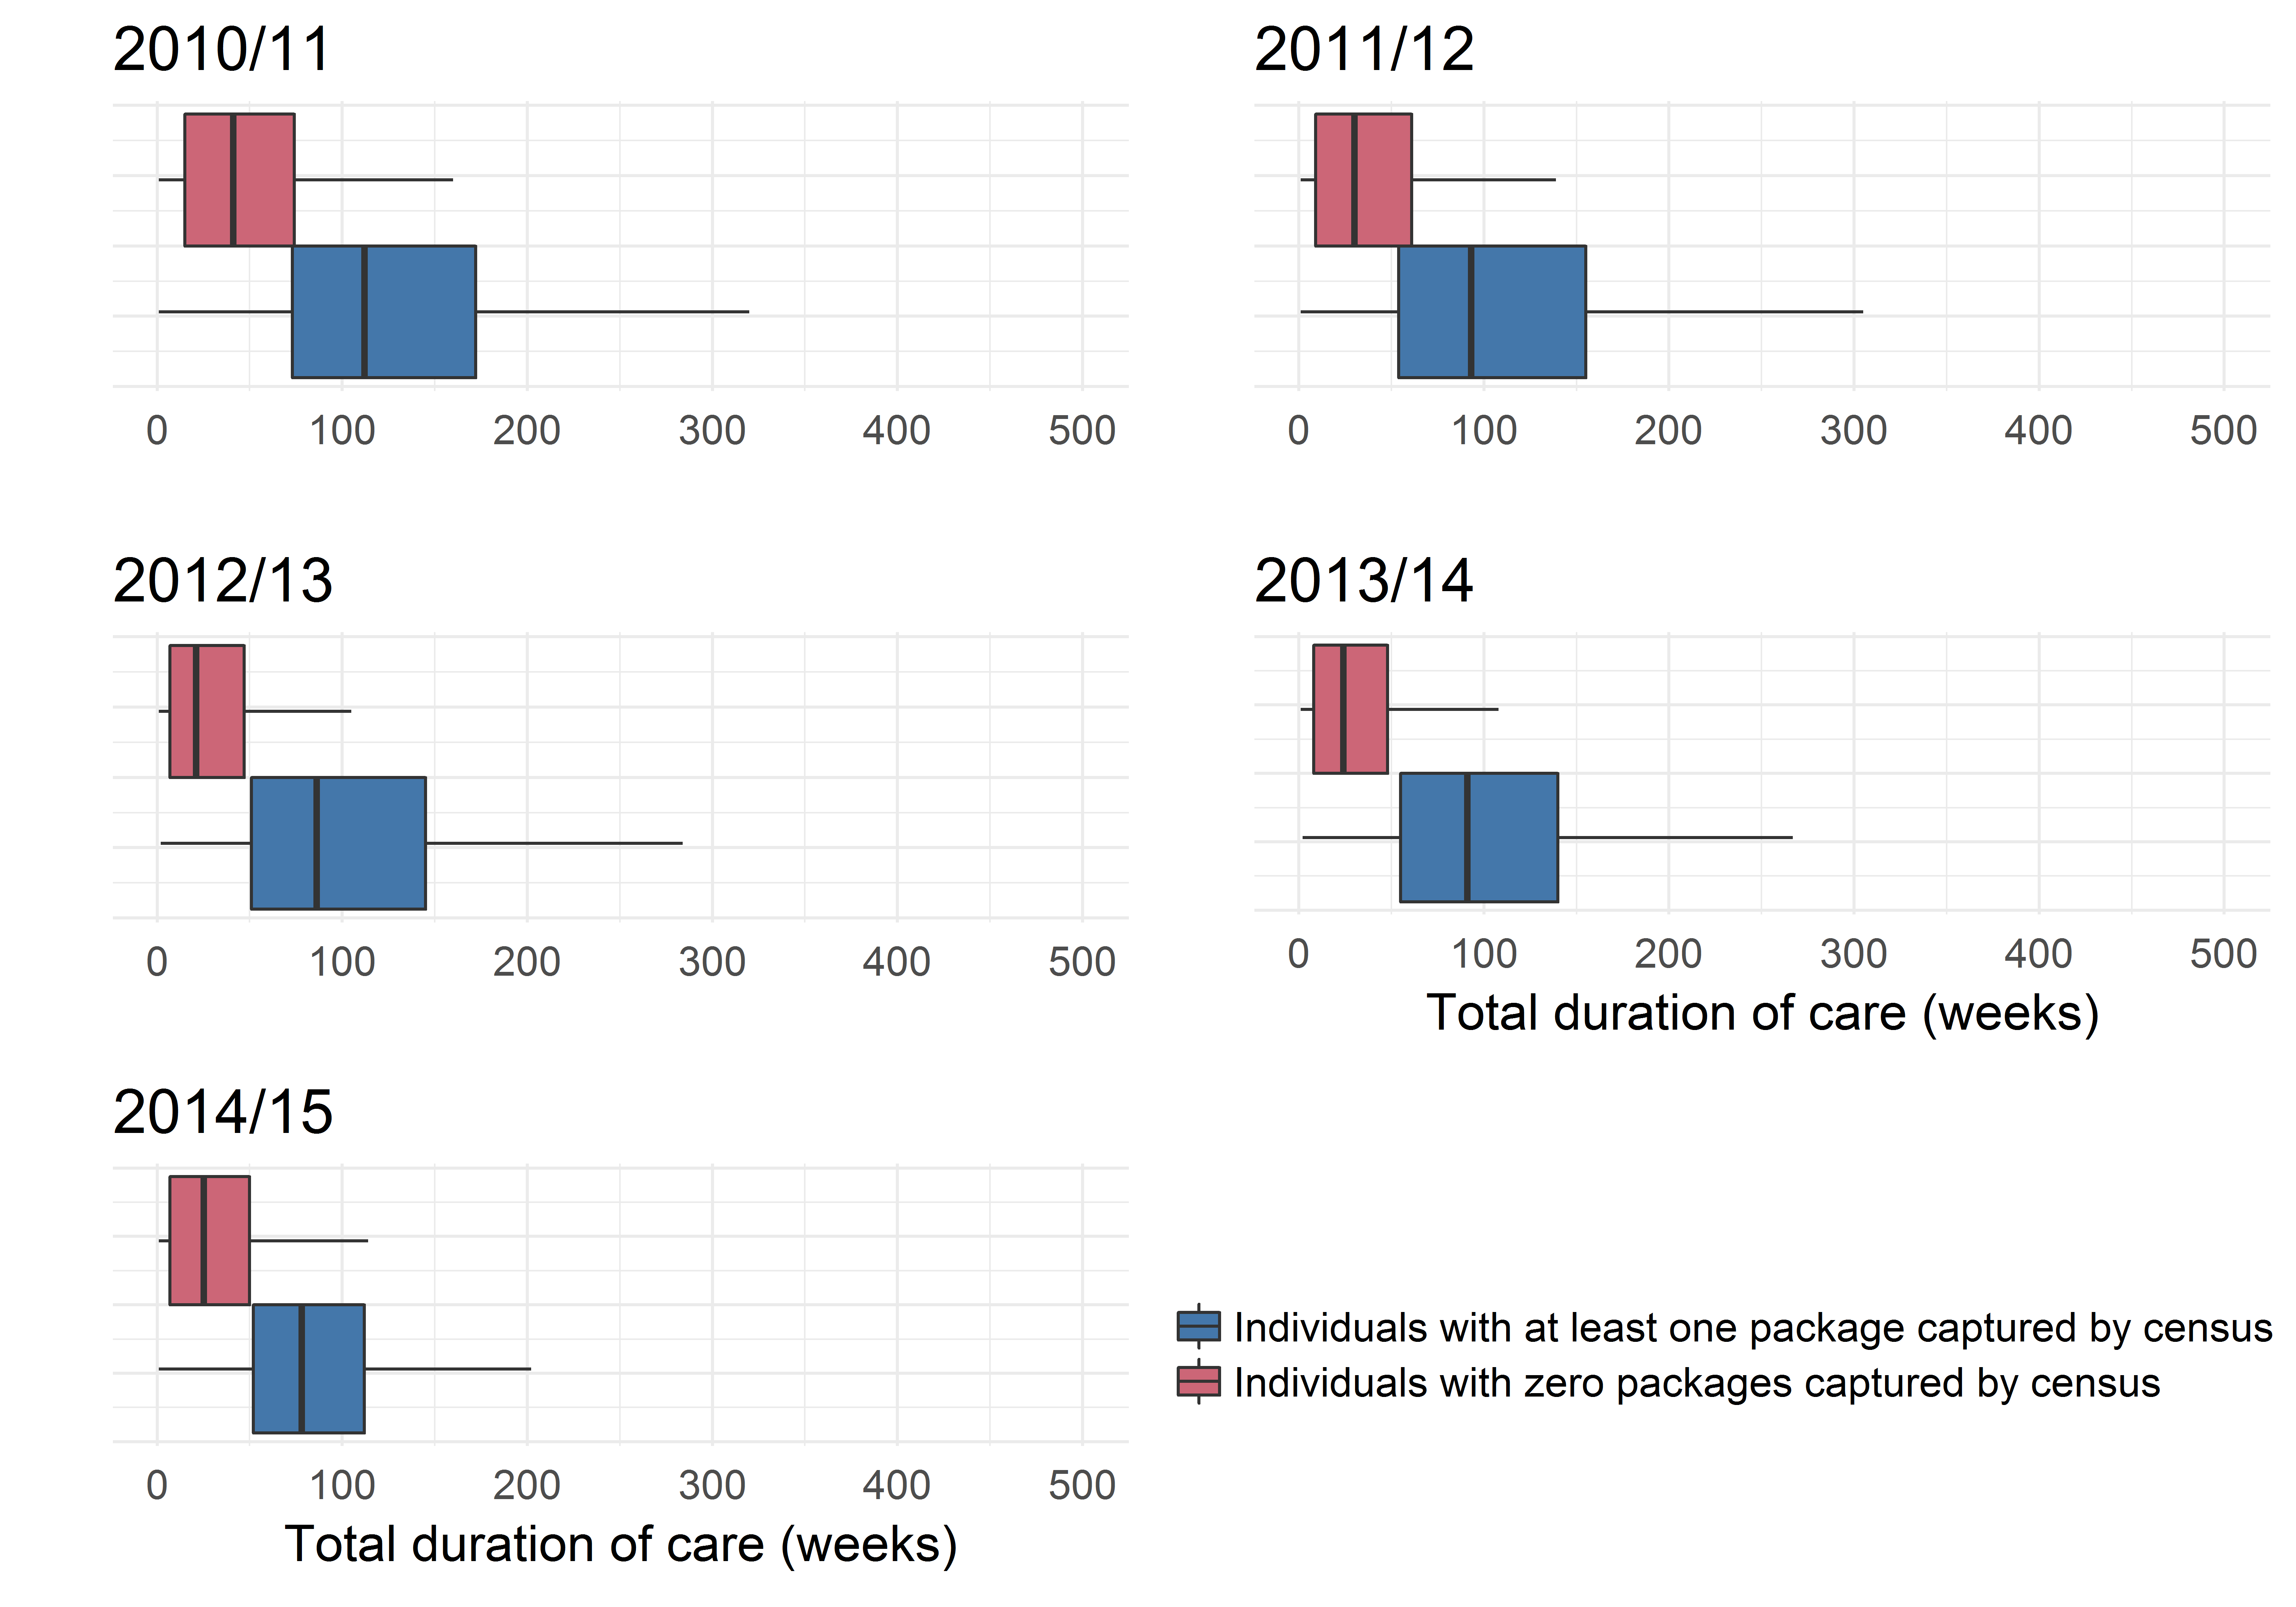
\includegraphics{figures/chapter-renf/17-duration.png}
    \caption{Variation in duration of home care}
    {\scriptsize outlying points removed to avoid disclosure}
    \label{fig:renf-duration}
\end{figure}

\begin{landscape}
\begin{longtable}[c]{@{}lllllllll@{}}
\caption{Regression models of package duration}
\label{tab:renf-regr-duration}\\
\toprule
\textbf{\begin{tabular}[c]{@{}l@{}}Financial\\ Year\end{tabular}} & \textbf{Gender} & \textbf{Age group} & \textbf{Type of home care} & \textbf{} & \textbf{estimate} & \textbf{std.error} & \textbf{statistic} & \textbf{p value} \\* \midrule
\endfirsthead
%
\multicolumn{9}{c}%
{{\bfseries Table \thetable\ continued from previous page}} \\
\toprule
\textbf{\begin{tabular}[c]{@{}l@{}}Financial\\ Year\end{tabular}} & \textbf{Gender} & \textbf{Age group} & \textbf{Type of home care} & \textbf{} & \textbf{estimate} & \textbf{std.error} & \textbf{statistic} & \textbf{p value} \\* \midrule
\endhead
%
\bottomrule
\endfoot
%
\endlastfoot
%
\textbf{2010/11} & \textbf{} & \textbf{} & \textbf{} & \textbf{(Intercept)} & \textbf{131.19} & \textbf{1.55} & \textbf{84.80} & \textbf{} \\
\textbf{} & \textbf{} & \textbf{} & \textbf{} & \textbf{No package in census} & \textbf{-76.55} & \textbf{2.62} & \textbf{-29.18} & \textbf{\textless{}0.05} \\
 & Female &  &  & (Intercept) & 132.62 & 1.83 & 72.40 &  \\
 & Female &  &  & No package in census & -75.29 & 3.20 & -23.54 & \textless{}0.05 \\
 & Male &  &  & (Intercept) & 127.36 & 2.89 & 44.12 &  \\
 & Male &  &  & No package in census & -78.09 & 4.59 & -17.01 & \textless{}0.05 \\
 &  & 65-75 &  & (Intercept) & 146.55 & 3.31 & 44.22 &  \\
 &  & 65-75 &  & No package in census & -98.60 & 5.68 & -17.35 & \textless{}0.05 \\
 &  & 76-85 &  & (Intercept) & 130.26 & 2.29 & 56.81 &  \\
 &  & 76-85 &  & No package in census & -73.53 & 3.89 & -18.89 & \textless{}0.05 \\
 &  & 86 plus &  & (Intercept) & 117.76 & 2.51 & 46.83 &  \\
 &  & 86 plus &  & No package in census & -60.34 & 4.21 & -14.32 & \textless{}0.05 \\
 &  &  & Care at home (Mainstream) & (Intercept) & 131.56 & 1.58 & 83.35 &  \\
 &  &  & Care at home (Mainstream) & No package in census & -76.67 & 2.67 & -28.77 & \textless{}0.05 \\
 &  &  & Rapid Response & (Intercept) & 140.74 & 7.85 & 17.92 &  \\
 &  &  & Rapid Response & No package in census & -90.23 & 14.54 & -6.21 & \textless{}0.05 \\
 &  &  & Reablement & (Intercept) & 17.57 & 5.87 & 2.99 &  \\
 &  &  & Reablement & No package in census & -11.24 & 13.98 & -0.80 & 0.43401 \\
 \\
 \\
 \\
\textbf{2011/12} & \textbf{} & \textbf{} & \textbf{} & \textbf{(Intercept)} & \textbf{111.31} & \textbf{1.44} & \textbf{77.39} & \textbf{} \\
\textbf{} & \textbf{} & \textbf{} & \textbf{} & \textbf{No package in census} & \textbf{-67.55} & \textbf{2.49} & \textbf{-27.09} & \textbf{\textless{}0.05} \\
 & Female &  &  & (Intercept) & 113.67 & 1.73 & 65.70 &  \\
 & Female &  &  & No package in census & -67.69 & 3.00 & -22.55 & \textless{}0.05 \\
 & Male &  &  & (Intercept) & 106.17 & 2.58 & 41.15 &  \\
 & Male &  &  & No package in census & -67.21 & 4.46 & -15.06 & \textless{}0.05 \\
 &  & 65-75 &  & (Intercept) & 122.75 & 2.72 & 45.06 &  \\
 &  & 65-75 &  & No package in census & -85.49 & 5.27 & -16.23 & \textless{}0.05 \\
 &  & 76-85 &  & (Intercept) & 109.74 & 2.25 & 48.73 &  \\
 &  & 76-85 &  & No package in census & -67.86 & 3.79 & -17.92 & \textless{}0.05 \\
 &  & 86 plus &  & (Intercept) & 101.08 & 2.49 & 40.60 &  \\
 &  & 86 plus &  & No package in census & -49.92 & 4.13 & -12.09 & \textless{}0.05 \\
 &  &  & Care at home (Mainstream) & (Intercept) & 117.92 & 1.58 & 74.84 &  \\
 &  &  & Care at home (Mainstream) & No package in census & -68.29 & 2.78 & -24.56 & \textless{}0.05 \\
 &  &  & Rapid Response & (Intercept) & 79.82 & 4.45 & 17.96 &  \\
 &  &  & Rapid Response & No package in census & -55.49 & 7.03 & -7.89 & \textless{}0.05 \\
 &  &  & Reablement & (Intercept) & 63.15 & 3.16 & 19.98 &  \\
 &  &  & Reablement & No package in census & -51.53 & 5.06 & -10.18 & \textless{}0.05 \\
 \\
 \\
 \\
\textbf{2012/13} & \textbf{} & \textbf{} & \textbf{} & \textbf{(Intercept)} & \textbf{104.68} & \textbf{1.20} & \textbf{87.51} & \textbf{} \\
\textbf{} & \textbf{} & \textbf{} & \textbf{} & \textbf{No package in census} & \textbf{-69.14} & \textbf{2.06} & \textbf{-33.51} & \textbf{\textless{}0.05} \\
 & Female &  &  & (Intercept) & 105.59 & 1.45 & 72.89 &  \\
 & Female &  &  & No package in census & -67.85 & 2.53 & -26.84 & \textless{}0.05 \\
 & Male &  &  & (Intercept) & 102.72 & 2.12 & 48.49 &  \\
 & Male &  &  & No package in census & -71.45 & 3.57 & -20.01 & \textless{}0.05 \\
 &  & 65-75 &  & (Intercept) & 120.31 & 2.73 & 44.05 &  \\
 &  & 65-75 &  & No package in census & -80.02 & 4.61 & -17.34 & \textless{}0.05 \\
 &  & 76-85 &  & (Intercept) & 102.25 & 1.77 & 57.92 &  \\
 &  & 76-85 &  & No package in census & -67.40 & 3.01 & -22.38 & \textless{}0.05 \\
 &  & 86 plus &  & (Intercept) & 95.62 & 1.87 & 51.00 &  \\
 &  & 86 plus &  & No package in census & -63.47 & 3.35 & -18.94 & \textless{}0.05 \\
 &  &  & Care at home (Mainstream) & (Intercept) & 117.05 & 1.52 & 77.20 &  \\
 &  &  & Care at home (Mainstream) & No package in census & -71.43 & 2.71 & -26.38 & \textless{}0.05 \\
 &  &  & Rapid Response & (Intercept) & 85.41 & 3.12 & 27.40 &  \\
 &  &  & Rapid Response & No package in census & -60.22 & 4.88 & -12.34 & \textless{}0.05 \\
 &  &  & Reablement & (Intercept) & 69.45 & 1.64 & 42.46 &  \\
 &  &  & Reablement & No package in census & -55.95 & 2.68 & -20.91 & \textless{}0.05 \\
 \\
 \\
 \\
\textbf{2013/14} & \textbf{} & \textbf{} & \textbf{} & \textbf{(Intercept)} & \textbf{104.94} & \textbf{1.09} & \textbf{95.88} & \textbf{} \\
\textbf{} & \textbf{} & \textbf{} & \textbf{} & \textbf{No package in census} & \textbf{-68.39} & \textbf{1.86} & \textbf{-36.75} & \textbf{\textless{}0.05} \\
 & Female &  &  & (Intercept) & 107.27 & 1.38 & 77.99 &  \\
 & Female &  &  & No package in census & -68.11 & 2.41 & -28.20 & \textless{}0.05 \\
 & Male &  &  & (Intercept) & 99.80 & 1.77 & 56.28 &  \\
 & Male &  &  & No package in census & -67.59 & 2.84 & -23.78 & \textless{}0.05 \\
 &  & 65-75 &  & (Intercept) & 121.50 & 2.42 & 50.14 &  \\
 &  & 65-75 &  & No package in census & -86.25 & 4.23 & -20.39 & \textless{}0.05 \\
 &  & 76-85 &  & (Intercept) & 103.77 & 1.62 & 63.93 &  \\
 &  & 76-85 &  & No package in census & -68.17 & 2.74 & -24.87 & \textless{}0.05 \\
 &  & 86 plus &  & (Intercept) & 91.45 & 1.69 & 53.97 &  \\
 &  & 86 plus &  & No package in census & -52.46 & 2.84 & -18.44 & \textless{}0.05 \\
 &  &  & Care at home (Mainstream) & (Intercept) & 114.43 & 1.46 & 78.32 &  \\
 &  &  & Care at home (Mainstream) & No package in census & -69.58 & 2.54 & -27.40 & \textless{}0.05 \\
 &  &  & Rapid Response & (Intercept) & 93.32 & 3.05 & 30.59 &  \\
 &  &  & Rapid Response & No package in census & -67.26 & 5.30 & -12.69 & \textless{}0.05 \\
 &  &  & Reablement & (Intercept) & 82.70 & 1.49 & 55.68 &  \\
 &  &  & Reablement & No package in census & -61.07 & 2.38 & -25.69 & \textless{}0.05 \\
 \\
 \\
 \\
\textbf{2014/15} & \textbf{} & \textbf{} & \textbf{} & \textbf{(Intercept)} & \textbf{90.76} & \textbf{0.99} & \textbf{91.86} & \textbf{} \\
\textbf{} & \textbf{} & \textbf{} & \textbf{} & \textbf{No package in census} & \textbf{-54.32} & \textbf{1.63} & \textbf{-33.23} & \textbf{\textless{}0.05} \\
 & Female &  &  & (Intercept) & 91.79 & 1.20 & 76.25 &  \\
 & Female &  &  & No package in census & -54.28 & 2.00 & -27.11 & \textless{}0.05 \\
 & Male &  &  & (Intercept) & 88.64 & 1.73 & 51.27 &  \\
 & Male &  &  & No package in census & -54.28 & 2.83 & -19.19 & \textless{}0.05 \\
 &  & 65-75 &  & (Intercept) & 106.95 & 2.30 & 46.56 &  \\
 &  & 65-75 &  & No package in census & -71.40 & 3.98 & -17.95 & \textless{}0.05 \\
 &  & 76-85 &  & (Intercept) & 84.83 & 1.34 & 63.13 &  \\
 &  & 76-85 &  & No package in census & -48.84 & 2.24 & -21.79 & \textless{}0.05 \\
 &  & 86 plus &  & (Intercept) & 85.24 & 1.68 & 50.62 &  \\
 &  & 86 plus &  & No package in census & -47.48 & 2.65 & -17.91 & \textless{}0.05 \\
 &  &  & Care at home (Mainstream) & (Intercept) & 98.60 & 1.40 & 70.59 &  \\
 &  &  & Care at home (Mainstream) & No package in census & -56.46 & 2.41 & -23.46 & \textless{}0.05 \\
 &  &  & Rapid Response & (Intercept) & 80.31 & 2.52 & 31.88 &  \\
 &  &  & Rapid Response & No package in census & -45.33 & 4.02 & -11.28 & \textless{}0.05 \\
 &  &  & Reablement & (Intercept) & 75.47 & 1.26 & 59.82 &  \\
 &  &  & Reablement & No package in census & -48.43 & 1.95 & -24.79 & \textless{}0.05 \\* \bottomrule
\end{longtable}
\end{landscape}

\begin{figure}[]
  \centering
    \includegraphics{figures/chapter-renf/19-dur-type-plot.png}
    \caption{Variation in duration of home care by care type}
    {\scriptsize outlying points removed to avoid disclosure}
    \label{fig:renf-dur-type}
\end{figure}

\FloatBarrier
\subsection{Variation in care packages captured by census}\label{subsec:renf-census-variation}

Descriptive statistics of the net difference in total hours of home care
for those individuals that have at least one package captured by the
census \emph{and} more than one package in a financial year are shown in
table \ref{tab:renf-net-diff}. The variation is plotted in figure
\ref{fig:renf-net-diff}. The median value of the net difference in total
hours of home care for individuals with multiple packages of ``Care at
home (Mainstream)'' is close to zero in all years with interquartile
ranges (IQR) varying from 4.25 to 8.5hrs. These individuals account for
approximately 60\% of all those captured by the census with multiple
packages of care.

The remaining individuals see larger negative values for the net
difference in total hours of home care over the financial year with
wider IQR values. Linear regression of the net difference in total hours
of homecare with home care type as an explanatory variable (table
\ref{tab:renf-net-diff-regr}) shows statistically significant results in
all years except 2010/11.

\vspace{3cm}

\begin{table}[h]
\centering
\resizebox{\textwidth}{!}{%
\begin{threeparttable}
\begin{tabular}{@{}llrrrrrrrr@{}}
\toprule
\textbf{\begin{tabular}[c]{@{}l@{}}Financial \\ Year\end{tabular}} & \textbf{Type of home care} & \textbf{\begin{tabular}[c]{@{}r@{}}number\\ of packages\end{tabular}} & \textbf{\begin{tabular}[c]{@{}r@{}}number \\ of unique\\ individuals\end{tabular}} & \textbf{mean} & \textbf{sd} & \textbf{median} & \textbf{IQR} & \textbf{\begin{tabular}[c]{@{}r@{}}25th\\ percentile\end{tabular}} & \textbf{\begin{tabular}[c]{@{}r@{}}75th\\ percentile\end{tabular}} \\ \midrule
2010/11 & Care at home (Mainstream) & 1456 & 561 & 0.23 & 5.01 & -0.13 & 4.25 & -2.00 & 2.25 \\
2010/11 & Rapid Response & 54 & 21 & -1.04 & 3.97 & -0.13 & 4.63 & -3.31 & 1.31 \\
2010/11 & Reablement\tnote{1} & * & * & -4.20 & 5.75 & 0.00 & 10.50 & -10.50 & 0.00 \\
2011/12 & Care at home (Mainstream) & 1241 & 437 & 0.73 & 5.52 & 0.25 & 5.25 & -1.75 & 3.50 \\
2011/12 & Rapid Response & 133 & 47 & -1.42 & 7.25 & -1.75 & 8.75 & -7.00 & 1.75 \\
2011/12 & Reablement & 119 & 38 & -5.52 & 5.28 & -5.25 & 7.00 & -10.00 & -3.00 \\
2012/13 & Care at home (Mainstream) & 1528 & 486 & 0.42 & 7.49 & 0.00 & 6.50 & -3.00 & 3.50 \\
2012/13 & Rapid Response & 242 & 72 & -2.55 & 7.33 & -2.50 & 10.75 & -8.75 & 2.00 \\
2012/13 & Reablement & 537 & 167 & -4.61 & 7.39 & -5.25 & 10.00 & -10.00 & 0.00 \\
2013/14 & Care at home (Mainstream) & 1648 & 498 & -0.37 & 7.50 & 0.00 & 8.00 & -4.50 & 3.50 \\
2013/14 & Rapid Response & 277 & 87 & -3.52 & 7.70 & -3.75 & 12.25 & -8.75 & 3.50 \\
2013/14 & Reablement & 672 & 209 & -2.52 & 8.80 & -3.50 & 13.00 & -9.50 & 3.50 \\
2014/15 & Care at home (Mainstream) & 1373 & 468 & 0.28 & 7.03 & 1.00 & 8.50 & -3.50 & 5.00 \\
2014/15 & Rapid Response & 241 & 73 & -1.94 & 10.29 & -3.50 & 14.00 & -10.50 & 3.50 \\
2014/15 & Reablement & 643 & 216 & -2.75 & 7.94 & -2.25 & 10.50 & -8.75 & 1.75 \\ \bottomrule
\end{tabular}
\begin{tablenotes}
\item[1] Numbers too low to be disclosed
\end{tablenotes}
\end{threeparttable}%
}
\caption{Variation in net difference of total hours of homecare by care type}
\label{tab:renf-net-diff}
\end{table}

\begin{figure}[]
  \centering
    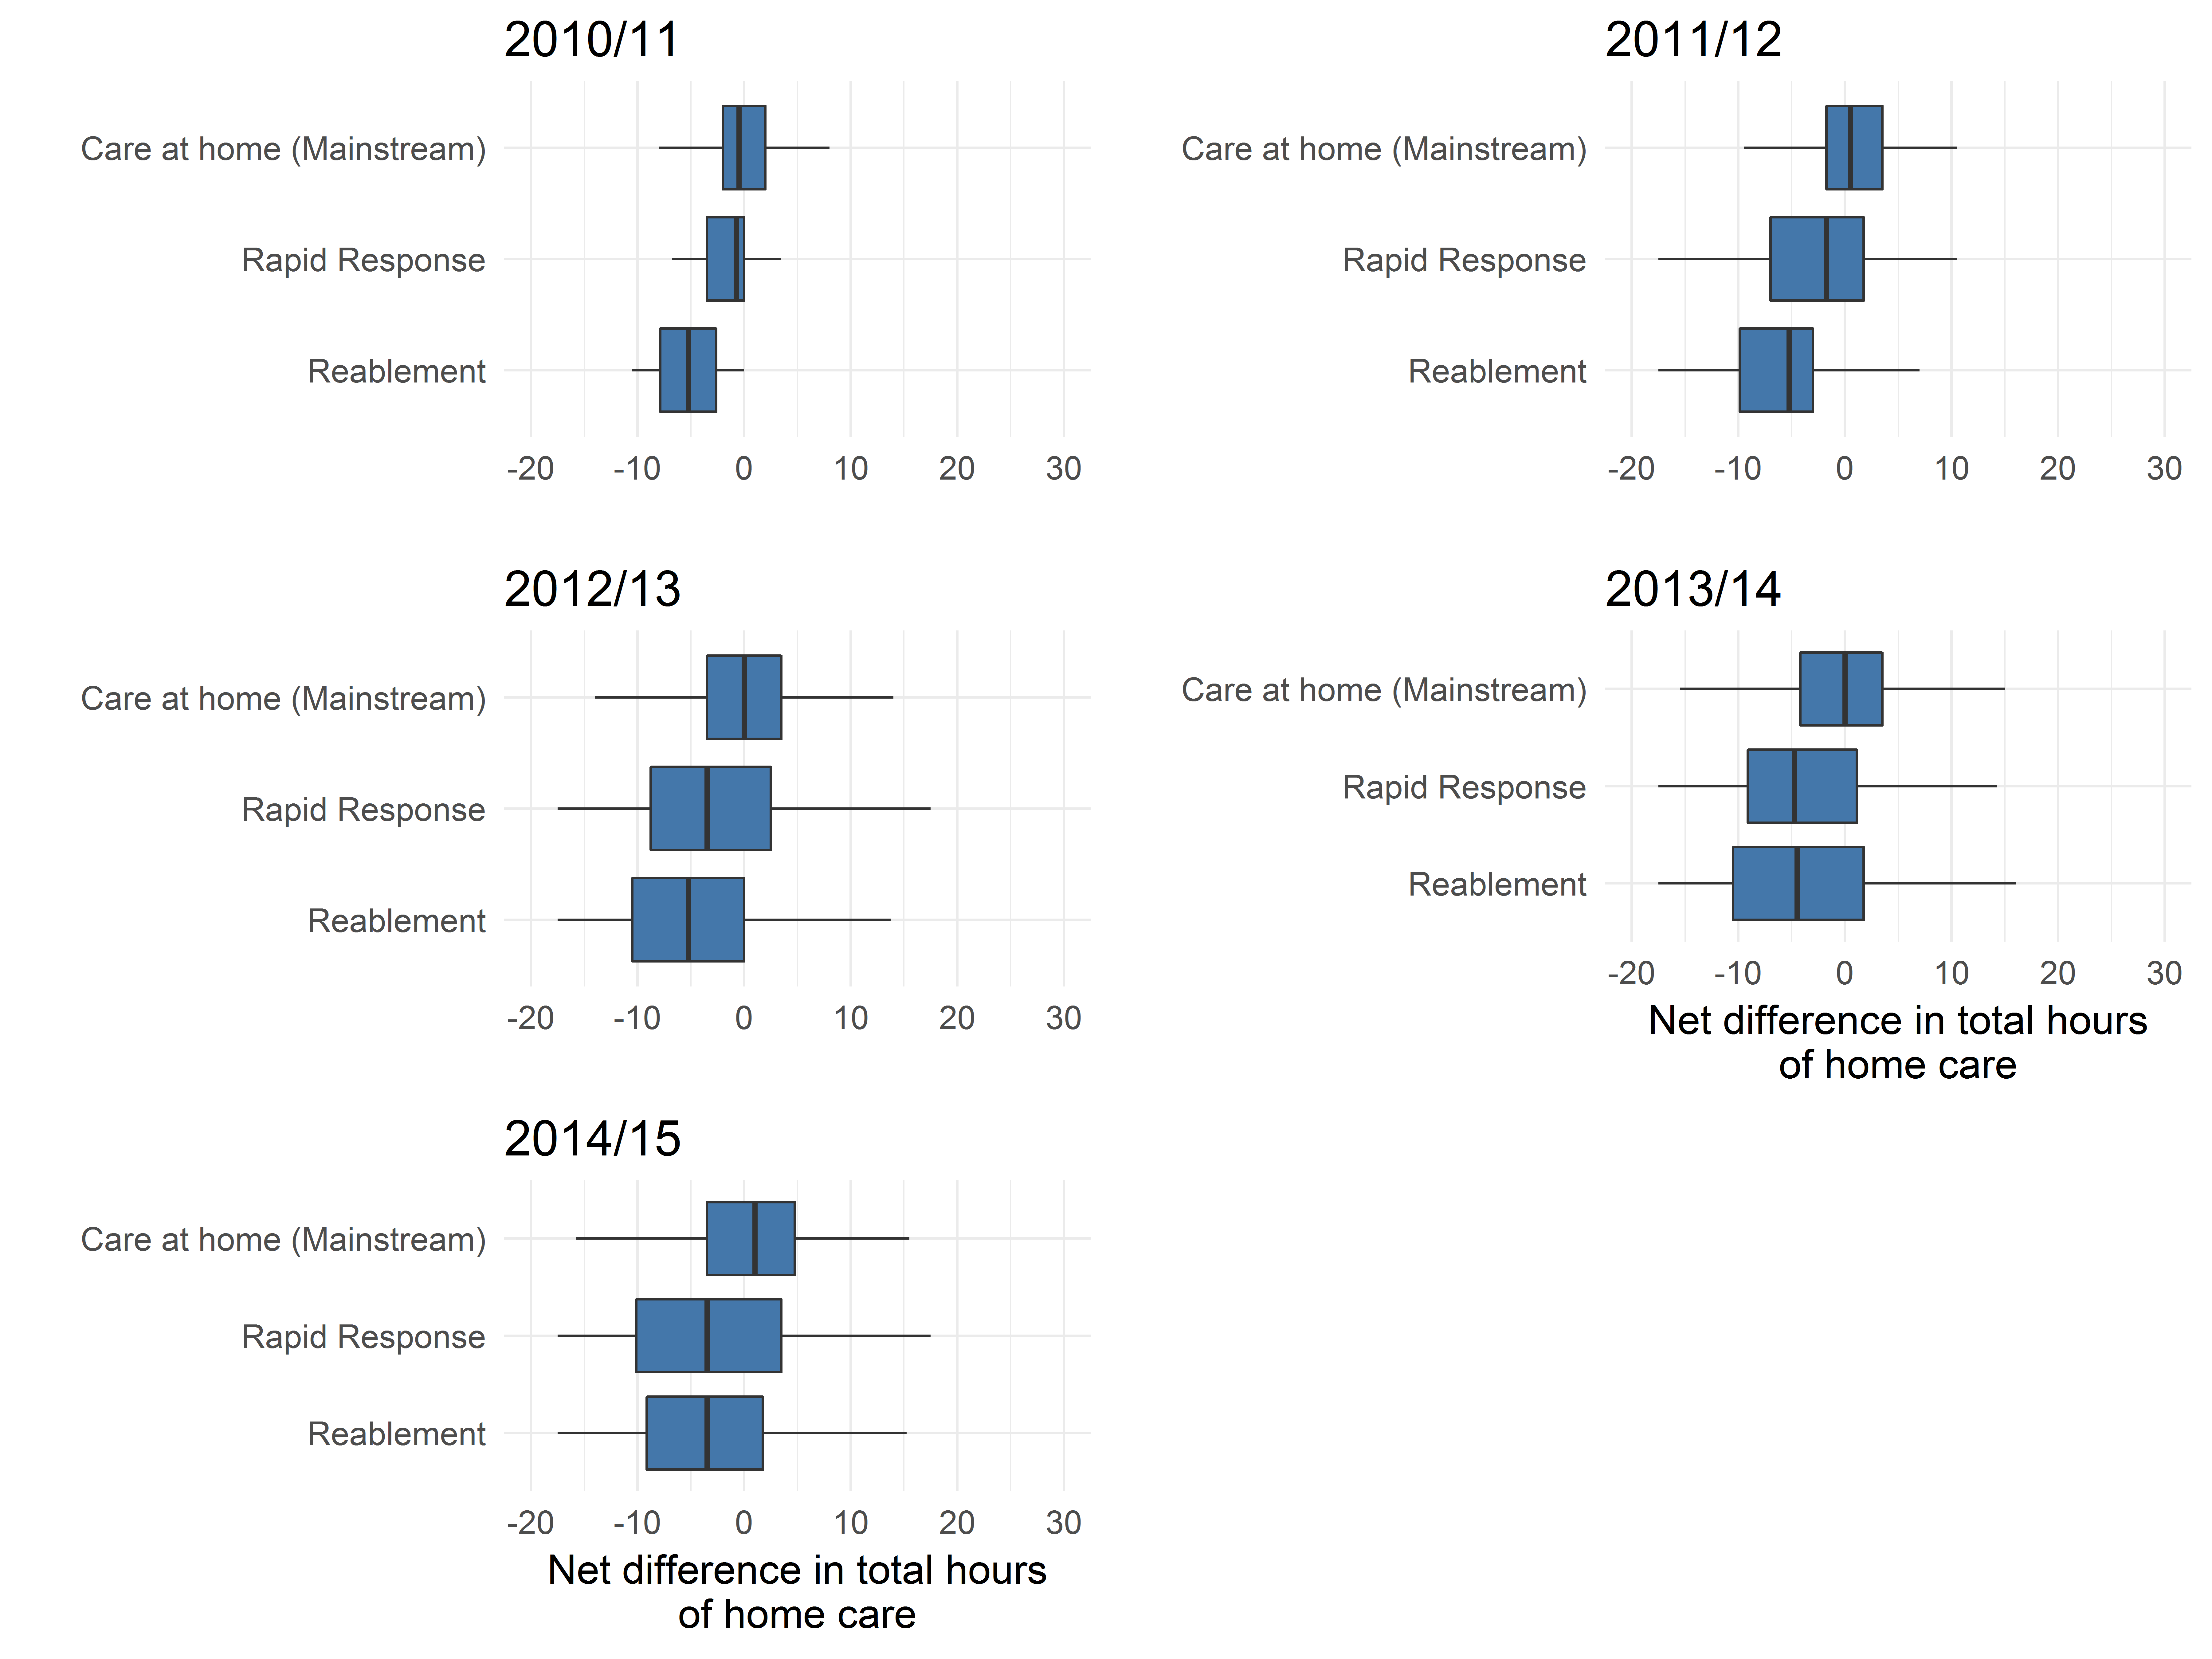
\includegraphics[]{figures/chapter-renf/10-net-diff-plot.png}
    \caption{Variation in net difference of total hours of care by care type}
    {\scriptsize outlying points removed to avoid disclosure}
    \label{fig:renf-net-diff}
\end{figure}

\begin{table}[]
\centering
\begin{tabular}{@{}llrrrr@{}}
\toprule
\textbf{\begin{tabular}[c]{@{}l@{}}Financial\\ Year\end{tabular}} & \textbf{} & \textbf{estimate} & \textbf{std.error} & \textbf{statistic} & \textbf{p value} \\ \midrule
\textbf{2010/11} & (Intercept) & 0.0562 & 0.1973 & 0.2846 &  \\
\textbf{} & Rapid Response & -1.3300 & 1.0386 & -1.2805 & 0.2009 \\
\textbf{} & Reablement & -5.3062 & 3.3102 & -1.6030 & 0.1095 \\
\textbf{2011/12} & (Intercept) & 0.7082 & 0.2739 & 2.5858 &  \\
\textbf{} & Rapid Response & -2.5433 & 0.8790 & -2.8936 & \textless{}0.05 \\
\textbf{} & Reablement & -6.2806 & 0.9684 & -6.4857 & \textless{}0.05 \\
\textbf{2012/13} & (Intercept) & 0.1091 & 0.3313 & 0.3292 &  \\
\textbf{} & Rapid Response & -2.9493 & 0.9222 & -3.1981 & \textless{}0.05 \\
\textbf{} & Reablement & -5.2183 & 0.6551 & -7.9661 & \textless{}0.05 \\
\textbf{2013/14} & (Intercept) & -0.4347 & 0.3440 & -1.2637 &  \\
\textbf{} & Rapid Response & -3.5078 & 0.8921 & -3.9321 & \textless{}0.05 \\
 & Reablement & -3.2064 & 0.6328 & -5.0675 & \textless{}0.05 \\
\textbf{2014/15} & (Intercept) & 0.0459 & 0.3481 & 0.1320 &  \\
 & Rapid Response & -2.3576 & 0.9476 & -2.4879 & \textless{}0.05 \\
 & Reablement & -3.5078 & 0.6194 & -5.6627 & \textless{}0.05 \\ \bottomrule
\end{tabular}
\caption{Regression models of net difference in total hours of care by home care type}
\label{tab:renf-net-diff-regr}
\end{table}

\FloatBarrier
\subsection{Multi-census}\label{subsec:renf-multi-census}

\begin{table}[h]
\centering
\resizebox{\textwidth}{!}{%
\begin{tabular}{@{}lccccc@{}}
\toprule
\textbf{Financial Year} & \textbf{\begin{tabular}[c]{@{}c@{}}Total receiving\\ home care (n)\end{tabular}} & \textbf{\begin{tabular}[c]{@{}c@{}}Captured by\\ census (\%)\end{tabular}} & \textbf{\begin{tabular}[c]{@{}c@{}}Captured by six-monthly\\ census (increase) (\%)\end{tabular}} & \textbf{\begin{tabular}[c]{@{}c@{}}Captured by four-monthly\\ census  (increase) (\%)\end{tabular}} & \textbf{\begin{tabular}[c]{@{}c@{}}Captured by three-monthly\\ census (increase)(\%)\end{tabular}} \\ \midrule
2006/07 & 2435 & 62.1 & 75.5 (13.4) & 80.9 (18.8) & 84.2 (22.1) \\
2007/08 & 2465 & 60.7 & 74.5 (13.8) & 80.1 (19.4) & 83.2 (22.4) \\
2008/09 & 2438 & 61.7 & 75.0 (13.3) & 81.3 (19.6) & 84.5 (22.8) \\
2009/10 & 2428 & 61.9 & 75.5 (13.7) & 81.1 (19.2) & 83.9 (22.0) \\
2010/11 & 2157 & 57.8 & 72.8 (15.0) & 82.9 (25.1) & 85.8 (28.0) \\
2011/12 & 2096 & 59.1 & 73.4 (14.3) & 78.9 (19.8) & 82.6 (23.5) \\
2012/13 & 2381 & 57.0 & 68.2 (11.3) & 73.9 (16.9) & 77.8 (20.8) \\
2013/14 & 2599 & 54.6 & 68.1 (13.5) & 73.7 (19.1) & 78.8 (24.2) \\
2014/15 & 2763 & 56.2 & 69.7 (13.5) & 86.6 (30.4) & 87.8 (31.6) \\ \midrule
\textbf{Mean}  & 2418 & 59.0 & 72.5 (13.5) & 79.9 (20.9) & 83.2 (24.2) \\ \bottomrule
\end{tabular}%
}
\caption{Proportion of individuals captured by census and hypothetical multi-census in each financial year}
\label{tab:renf-multi-census}
\end{table}

Table \ref{tab:renf-multi-census} shows the percentage of the total
number of individuals receiving home care in each financial year that
would be captured if six-monthly, four monthly, or three-monthly census
had been conducted and the increases these would signify. A bi-annual
census would have captured an average of 72.5\% of individuals that
received home care during the study period - an average increase of
13.5\% from the census. Tri-annual census collection would have captured
an average 79.9\% of individuals (average increase of 20.9\%) whilst a
quarterly census collection would have captured an average 83.2\% of
individuals (average increase of 24.2\%).

The largest increases are seen in the years where the number of
individuals captured by a single census are relatively low compared to
other years, in particular 2010/11, 2013/14, and 2015/16.

\section{Discussion}\label{sec:renf-discuss}

\subsection{Findings}\label{subsec:renf-discuss-find}

This exploratory project has investigated the variation in packages of
care from one Scottish local authority area and aimed to: a) quantify
the proportion of individuals in receipt of home care during Social Care
Survey census week, b) describe the differences in individuals that
receive some care during the census week and those that don't, c)
validate the value of total weekly hours of care compared to the rest of
the financial year for those that \emph{do} receive some care during the
census, and d) assess the difference in the proportion of individuals
that would be captured by hypothetical extra census dates.

Between 51.7\% and 61.9\% of all individuals receiving home care in the
years 2006/07 to 2015/16 had ``live'' packages of care during the SCS
census week. The trend is decreasing with the minimum value being
recorded in the most recent year of data. This trend likely reflects the
increase seen in the proportion of ``Reablement'' type packages of care
which are designed to be implemented for short periods of time following
hospital discharge. The shorter duration of these packages means they
are less likely to coincide with the census date. There are no
significant differences in the overall proportion or demographic
structure of the group that are not captured by the census compared to
the group that are in each financial year.

Individuals that have no packages of home care captured by the census in
each year have a considerably shorter total duration of care. This is
seen across all care types and age and gender groups. The most likely
explanation for this is that no matter what care type, some individuals
go on to require longer term care and thus receive more contiguous
packages which eventually coinciding with a census date. Those that have
zero packages captured by a census truly are short-term users of care.
It is impossible, with this data, to account for what proportion of this
is due to care no longer being required, to mortality, or to other
causes.

Those without any packages captured by a census are also more likely to
have slightly more total hours of home care per week. This is a moderate
increase and affects individuals receiving ``Reablement'' type care to a
greater extent. The difference for individuals receiving ``Care at home
(Mainstream)'' type packages (the large majority) is equivalent to, on
average, 10 minutes per day extra care.

For approximately 50\% of individuals that \emph{do} have at least one
package of care captured by a census - the value of total weekly hours
of home care that they receive in the census week is absolutely
representative. This is because they only receive one package of care
during the financial year and are likely recipients of long-term care.
\textbf{Make sure the results show this clearly}

The remaining individuals receive multiple packages of care during the
financial year or stop receiving care altogether. There are differences
in the variation in the net-difference of total hours of home care for
these individuals depending on the type of care they receive.
Individuals with ``Care at home (Mainstream)'' type packages (again a
majority\textbf{how much??}) show mild variation with median values
close to zero. Half of these packages in 2014/15 (the year with the
widest IQR) see a net difference value between -30 minutes to +40
minutes of care per day.

Those receiving ``Reablement'' or ``Rapid Response'' type packages
(\textbf{quantify}) are more likely to have negative net difference
values. It is possible these are short-term packages of care that
started soon before the census and end soon after resulting in negative
values. The IQR in 2014/15 indicates half of these packages see
variations of care between -75 or -90 to +15 or +30 minutes of care per
day respectively.

Adding an additional 1, 2, or 3 census weeks in each financial year to
the data analysed in this project increases the proportion of
individuals that would be surveyed by an average of 13.5\%, 20.9\%, or
24.2\% to 72.5\%, 79.9\%, or 83.2\% respectively.

\subsection{Limitations}\label{subsec:renf-discuss-lim}

This analysis is limited by the fact that data was obtained from only
one local authority area. It is impossible to know if the number of
individuals captured or not by the SCS in the Renfrewshire area is
indicative of numbers across the country. Given each of the 32 local
authorities in Scotland have bespoke methods of delivering and recording
social care the findings from this analysis can not be generalised to a
national level. However, given the difficulties in obtaining data of
this kind, the analysis gives some indication to stakeholders of the
validity of the SCS.

Furthermore, the method of summarising data into packages of care is
subjective and may differ from the method used by Renfrewshire council
to complete the SCS. Absolute numbers of individuals receiving home care
in each financial year in this analysis are similar to those returned by
Renfrewshire council to the SCS overall with some mild discrepancy in
later years. Eligibility to be included in the home care census has
changed over the years (e.g. ``Housing Support'' being included as home
care and then collected as a separate type of service in later years)
and the collection of individual-level data did not begin until 2010/11.
Whether this has changed how data is collated at the local level for
return to SCS is unknown but may explain differences in counts.

\textbf{Did not account for SEP}

\subsection{Implications}\label{subsec:renf-discuss-imp}

The analysis in this chapter suggests the SCS provides a good
cross-sectional sample of individuals receiving home care in any given
financial year. The proportion of this sample appears to be decreasing
in more recent years but still accounts for at least half of all
individuals receiving care.

Increasing the frequency of data collection to four times a year could
potentially increase the sample size to approximately 83\%. Whether the
extra administrative resources associated with this would be too great
for both local authority and Scottish Government analytical teams is a
matter which would require further consideration. This would certainly
result in more short-term packages of care being captured by data
collection enhancing the representativeness of the SCS.

The value of total hours of home care returned to the SCS is an accurate
cross-sectional value but is not completely indicative of care received
throughout a financial year. A majority of individuals have no, or only
a modest, variation in the total weekly hours of home care they receive
during a financial year. However, a proportion of individuals
(\textbf{25\%??}) have large changes in total hours of homecare and
these cannot be indented in SCS data. The main analysis in this thesis,
and any other research using the SCS as a data source, cannot infer home
care receipt over a year from this value as it risks producing biased
results. Collection of start and end dates of all home care packages
received in a financial year in the SCS would rectify this problem.

The analysis of the data from Renfrewshire council has shown there are
different patterns in the duration and intensity of home care packages
according to the type of care being provided (e.g.~between ``Care at
home (Mainstream)'' and ``Rapid Response'' type packages). The SCS does
not collect data on the categorisation of care type and therefore these
differences cannot be accounted for in research using the SCS. Adding a
standardised classification of home care type to the SCS would allow a
richer interpretation of home care users for both official statistical
reporting and research purposes.

\subsection{Future work}\label{subsec:renf-discuss-future}

Future work using this data should consider the difference in
individuals receiving care at different time intervals (e.g.~first six
months of the year). If the census week were to capture a higher
proportion of individuals in a more narrow time-frame then alternative
types of statistical analyses, such as time-to-event analysis, may be
possible using SCS data.\\
The data from Renfrewshire council also offers the opportunity to
longitudinally analyse home care use by age, gender, and type of home
care groups. Quantifying any differences in the change over time in the
amount of home care used would be of interest to both researchers and
local authority providers.

Each individual in the dataset has data with multiple values of Scottish
Index of Multiple Deprivation (SIMD) for different time periods. Future
analysis should include this variable with the correct SIMD score added
to the time series at the appropriate time period. Accounting for
socioeconomic position in all analyses would provide a richer picture of
service allocation. Time constraints prevented such analysis in this
chapter.

\section{Conclusion}\label{sec:renf-conc}

Analysis of individual level social care data from Renfrewshire council
area suggests that the number of people recorded as receiving home care
by the Social Care Survey captures between 52\% and 62\% of the total
number of people that will receive home care during a financial year.
Those not captured during a census week are individuals receiving
short-term care only. The value of total weekly hours of home care
recorded during the census week, whilst an accurate cross-sectional
figure, is not an accurate representation of care receipt over the whole
financial year for a small proportion of individuals. Collection of
additional data, such as start and stop dates for all packages of care
and type of home care delivered, would improve the inferences that can
be made from the SCS currently.

\hypertarget{refs}{}
\hypertarget{ref-RN527}{}
Arnold, JB, G Daroczi, B Werth, B Weitzner, J Kunst, B Auguie, B Rudis,
H Wickham, J Talbot, and J London. 2018. ``Ggthemes: Extra Themes,
Scales, and Geoms for `Ggplot2'. R Package Version 3.5.0.'' Report.
\url{https://CRAN.R-project.org/package=ggthemes}.

\hypertarget{ref-RN526}{}
Bache, S.M., and H Wickham. 2014. ``Magrittr:A Forward Pipe Operator for
R. R Package Version 1.5.'' Report.
\url{https://CRAN.R-project.org/package=magrittr}.

\hypertarget{ref-RN356}{}
Dancho, M., and D. Vaughan. 2017. ``Tibbletime:Time Aware Tibbles. R
Package Version 0.0.2.'' Report.
\url{https://CRAN.R-project.org/package=tibbletime}.

\hypertarget{ref-RN522}{}
Grolemund, G., and H Wickham. 2017. ``Lubridate:Dates and Times Made
Easy with Lubridate. R Package Version 1.6.0.'' Report.
\url{https://CRAN.R-project.org/package=lubridate}.

\hypertarget{ref-RN523}{}
Henry, L., and H Wickham. 2017. ``Purrr:Functional Programming Tools. R
Package Version 0.2.4.'' Report.
\url{https://CRAN.R-project.org/package=purrr}.

\hypertarget{ref-RN500}{}
ISD. 2017. ``Revised Source Social Care Dataset. Definitions and
Recording Guidance. (Draft Nov 2017 Version 1.4).'' Report.
\url{http://www.isdscotland.org/Health-Topics/Health-and-Social-Community-Care/docs/Proposed-SC-Definitions-Recording-Guidance-v1-3-Draft.doc}.

\hypertarget{ref-RN492}{}
NRS. 2015. ``Renfrewshire Coucnil Area - Demographic Factsheet.''
Report.
\url{https://www.nrscotland.gov.uk/files/statistics/council-area-data-sheets/renfrewshire-factsheet.pdf}.

\hypertarget{ref-RN295}{}
R-Core-Team. 2017. ``R: A Language and Environment for Statistical
Computing. R Foundation for Statistical Computing.'' Report.
\url{http://www.R-project.org}.

\hypertarget{ref-RN495}{}
Renfrewshire-Council. 2015. ``Corporate Records Management Policy.''
Report.
\url{http://www.renfrewshire.gov.uk/media/2763/Records-Management-Policy/pdf/App4-RecordsManagementPolicyv3.0-20151111.pdf}.

\hypertarget{ref-RN520}{}
Robinson, D. 2017. ``Broom: Convert Statistical Analysis Objects into
Tidy Data Frames. R Package Version 0.4.2.'' Report.
\url{https://CRAN.R-project.org/package=broom}.

\hypertarget{ref-RN498}{}
RStudio-team. 2016. ``Integrated Development for R. Rstudio, Inc.,
Boston, Ma. Version 1.0.143.'' Report.
\href{\%20http://www.rstudio.com/}{http://www.rstudio.com/}.

\hypertarget{ref-RN494}{}
Scottish-Government. 2017a. ``SIMD2016 Local Share Tool.'' Report.
\url{http://www.gov.scot/Resource/0051/00515034.xlsx}.

\hypertarget{ref-RN499}{}
---------. 2017b. ``Social Care Services, Scotland, 2017.'' Report.
\url{http://www.gov.scot/Publications/2017/12/3849/downloads}.

\hypertarget{ref-RN487}{}
---------. 2017c. ``Social Care Survey.'' Report.
\url{http://www.gov.scot/Topics/Statistics/Browse/Health/Data/HomeCare}.

\hypertarget{ref-RN521}{}
Wickham, H. 2017. ``Forcats:Tools for Working with Categorical Variables
(Factors). R Package Version 0.2.0.'' Report.
\url{https://CRAN.R-project.ork/package=forcats}.

\hypertarget{ref-RN525}{}
Wickham, H, and W. Chang. 2016. ``Ggplot2:Create Elegant Data
Visualisations Using the Grammer of Graphics. R Package Version 2.2.1.''
Report. \url{https://CRAN.R-project.org/package=ggplot2}.

\hypertarget{ref-RN524}{}
Wickham, H, and L. Henry. 2017. ``Tidyr:Easily Tidy Data with `Spread()`
and `Gather()` Functions. R Package Version 0.7.2.'' Report.
\url{https://CRAN.R-project.org/package=tidyr}.

\hypertarget{ref-RN283}{}
Wickham, Hadley, and Romain Francois. 2017. ``Dplyr: A Grammar of Data
Manipulation. R Package Version 0.7.4.'' Report.
\url{https://CRAN.R-project.org/package=dplyr}.


\end{document}
